\chapter{条件期望、线性投影与回归模型}
\label{ch:U02-cef}

本章回答一个最基本的问题：写下 $y_i=x_i\T\beta+u_i$ 时，$\beta$ 和 $u_i$ 究竟是什么？答案分三层：(1) 任何一对随机变量 $(y,x)$ 都可分解为“条件期望 $+$ 误差”，$y=\E(y\mid x)+u$，且自动满足 $\E(u\mid x)=0$（CEF 分解）；(2) 条件期望恰好线性时得到线性回归模型；不线性时仍可定义“最佳线性预测”（线性投影），它总存在，但误差只满足较弱的 $\E(xu)=0$；(3) $\beta$ 能否解释为因果效应，需要条件独立（外生性）等额外假设。本章是全书的“总体层面”基础：第 1 章给出了条件期望的工具性质，本章把它们用于回归模型；第 3 章把这里的总体矩换成样本矩得到 OLS，第 4、5 章研究 OLS 的有限样本与大样本性质，第 7--8 章处理 $\E(u\mid x)\neq0$（内生性）。学习路线：先掌握 CEF 分解与迭代期望律（第 \ref{sec:U02-cef}--\ref{sec:U02-err} 节），再学最优预测、条件方差与系数解释，最后学线性投影、遗漏变量偏误与因果效应。对应 Hansen 第 2 章（Conditional Expectation and Projection）。

%======================================================================
\section{截面数据与模型的基本要素}\label{sec:U02-basics}

本节交代数据的形式、全书记号，以及模型中哪些量可观测、哪些不可观测、哪些是待估参数。

\subsection{截面数据 \texorpdfstring{$(y_i,x_i)$}{(y\_i, x\_i)}：样本与总体}

\subsubsection{截面数据的定义与记号}

\term{截面数据}{cross-sectional data}是在同一时点（或同一时期）对 $n$ 个个体（人、企业、地区）各观测一次得到的数据。截面模型的出发点就是这样一组观测：
\[
(y_i,\ x_i),\qquad i=1,2,\dots,n,
\]
其中 $y_i$ 是标量\term{被解释变量}{dependent variable}（又称因变量、响应变量），$x_i$ 是 $K\times1$ 的\term{解释变量}{regressors}向量（又称自变量、回归元）。

\subsubsection{用样本推断总体}

计量经济学的基本思路：把样本看作从某个\term{总体}{population}中抽出的随机变量的实现值，用样本推断总体。例如，用一个“工资—教育”样本学习总体中工资（wage）与教育（educ）的关系。样本如何抽取（是否 \iid）是第 4 章假设 A2 的内容；本章只在总体层面讨论 $(y,x)$ 的联合分布，下标 $i$ 常省略。

\subsection{记号约定：本书与 Hansen 的对照}

\subsubsection{记号对照表}

不同教材记号不一，考场上看到任何一种都要认得。

\begin{center}
\small
\begin{tabularx}{\linewidth}{lllL}
\toprule
对象 & 本书 & 其他常见写法 & Hansen\\
\midrule
误差项 & $u_i$ & CEF 分解中写 $v_i$ & $e_i$\\
条件期望函数 & $\E(y_i\mid x_i)$ & --- & $m(x)=\E[Y\mid X=x]$\\
随机变量 & 小写 $y_i,x_i$ & 小写 & 大写 $Y,X$；小写表示取值\\
回归元个数 & $K$（含常数项） & $K$ 只计斜率个数 & $k$\\
转置 & $x\T$ & $x^\top$ & $x'$\\
真值 & $\beta$ & $\beta_0$（下标 0 表示真值） & $\beta$\\
\bottomrule
\end{tabularx}
\captionof{table}{本章记号对照}
\end{center}

\subsubsection{\texorpdfstring{$K$}{K} 是否包含截距：自由度公式的陷阱}

\begin{note}[$K$ 是否包含截距]
线性模型常写成 $y_i=\beta_0+x_{i1}\beta_1+\cdots+x_{iK}\beta_K+u_i=x_i\T\beta+u_i$，严格说这有 $K+1$ 个参数；而同时又说数据矩阵 $X$ 是 $n\times K$ 的，二者矛盾。\key{本书约定}：$x_i$ 是 $K\times1$ 向量，且第一个元素恒为常数 1，所以参数个数为 $K$，残差自由度为 $n-K$。若采用另一种约定（$K$ 个斜率 $+$ 1 个截距），自由度写作 $n-K-1$，第 6 章 $F$ 检验公式中的 $n-K-1$ 就来自这种约定。两者只是 $K$ 的定义不同，答题时先写清楚你的 $K$ 是否含截距。
\end{note}

\subsection{可观测量、不可观测量与待估参数}

\subsubsection{三类对象：数据、误差、参数}

写出模型 $y_i=x_i\T\beta+u_i$ 后，必须分清三类对象：
\begin{itemize}
  \item $(y_i,x_i)$：\term{可观测}{observed}，是数据。其中 $x_i$ 由研究者选择与构造（取对数、平方、交互项等）。
  \item $u_i$：\term{不可观测}{unobserved}，只能通过 $u_i=y_i-x_i\T\beta$ 间接“看到”。
  \item $\beta$：未知但固定的\term{感兴趣参数}{parameter of interest}，是估计的目标。
\end{itemize}

\subsubsection{误差不可观测，故选 \texorpdfstring{$\beta$}{beta} 使隐含误差最小：OLS 的出发点}

$u_i$ 看不见，但对任一候选值 $b$，“隐含的误差” $y_i-x_i\T b$ 是可以算出来的。于是自然的做法是：选 $b$，使隐含误差整体上尽量小（例如平方和最小）。这正是第 3 章 OLS 的出发点；本章第 \ref{sec:U02-blp} 节的线性投影是它的总体版本。

\begin{english}
We observe a cross-sectional sample $\{(y_i,x_i)\}_{i=1}^n$, where $y_i$ is the dependent variable and $x_i$ is a $K\times1$ vector of regressors including a constant. In the model $y_i=x_i'\beta+u_i$, $(y_i,x_i)$ are observed, the error $u_i$ is unobserved, and $\beta$ is the unknown (fixed) parameter of interest. Since $u_i$ is unobserved, we choose $\beta$ to make the implied errors $y_i-x_i'\beta$ as small as possible.
\end{english}

%======================================================================
\section{两类模型：非参数模型与线性模型}\label{sec:U02-models}

刻画 $y$ 与 $x$ 的关系有两条路：不设函数形式（非参数模型），或设定为对参数线性（线性模型）。本节比较二者的得失。

\subsection{非参数模型 \texorpdfstring{$y_i=f(x_i)+u_i$}{y\_i = f(x\_i) + u\_i}：灵活但计算困难}

\subsubsection{定义与“灵活”的含义}

\term{非参数模型}{nonparametric model}不对函数形式作参数化假定：
\[
y_i=f(x_i)+u_i,
\]
$f(\cdot)$ 是未知函数，只要求满足一定光滑性。好处是\key{灵活}（flexible）：$f$ 可以先升后降再陡升（见图 \ref{fig:U02-np}），不会因函数形式设错而产生\term{设定误差}{misspecification}。

\subsubsection{“计算困难”与维数灾难}

代价是\key{计算困难}（computationally difficult）：要估计的是整条曲线（无穷维对象），而不是有限个参数。更严重的是\term{维数灾难}{curse of dimensionality}：$x$ 的维数 $d$ 越大，同样样本量下落在某点 $x$“附近”的观测越稀少，估计精度急剧下降。

\begin{extend}[维数灾难的收敛速度]
用二阶核、$f$ 二阶可导时，核估计在一点处的偏差约为 $O(h^2)$，方差约为 $O\big(1/(nh^d)\big)$（$h$ 为带宽，见下一小节）。均方误差 $\approx c_1h^4+c_2/(nh^d)$；令两项同阶，$h^4\asymp 1/(nh^d)$，得 $h\asymp n^{-1/(4+d)}$，最优均方误差的收敛速度为
\[
n^{-4/(4+d)}.
\]
$d=1$ 时为 $n^{-4/5}$；$d$ 增大则越来越慢，远慢于参数模型的 $n^{-1}$。
\end{extend}

\subsection{非参数估计方法一：核估计}

\subsubsection{局部加权平均与 Nadaraya--Watson 估计量}

\term{核估计}{kernel estimation}的思想是“局部加权平均”：估计 $f(x)$ 时只用 $x_i$ 落在 $x$ 附近的观测，越近权重越大。最常见的 \term{Nadaraya--Watson 估计量}{Nadaraya-Watson estimator}为
\[
\hat f(x)=\frac{\sum_{i=1}^nK\!\left(\frac{x_i-x}{h}\right)y_i}{\sum_{i=1}^nK\!\left(\frac{x_i-x}{h}\right)},
\]
其中 $K(\cdot)$ 是核函数（如标准正态密度），$h>0$ 是\term{带宽}{bandwidth}。分母使权重之和为 1，所以 $\hat f(x)$ 是 $y_i$ 的加权平均。

\subsubsection{带宽 \texorpdfstring{$h$}{h} 的偏差—方差权衡}

$h$ 大 $\Rightarrow$ 平均范围宽、曲线平滑：偏差大、方差小；$h$ 小则相反。带宽选择是核估计的核心难点。详见 Hansen 第 19 章。

\subsection{非参数估计方法二：级数（筛）估计}

\subsubsection{用有限个基函数逼近未知函数}

\term{级数估计}{series estimation}（又称\term{筛估计}{sieve estimation}）用有限个基函数逼近 $f$：
\[
f(x)\approx\gamma_0+\gamma_1p_1(x)+\cdots+\gamma_Jp_J(x),
\]
例如多项式基 $p_j(x)=x^j$ 或样条。给定 $J$，这就是一个对参数线性的回归，可直接用 OLS 估计 $\gamma$（第 3 章）；理论上令 $J\to\infty$ 随 $n$ 缓慢增长，近似误差趋于 0。

\subsubsection{陈晓红与筛估计理论}

核估计与级数估计是非参数估计的两大方法。级数（筛）估计大样本理论的代表人物是耶鲁大学经济学教授陈晓红（Xiaohong Chen），其综述见 Chen (2007)，载 \textit{Handbook of Econometrics} 第 6B 卷。

\subsection{线性模型 \texorpdfstring{$y_i=x_i\T\beta+u_i$}{y\_i = x\_i'beta + u\_i} 与误差项的含义}

\subsubsection{线性模型的形式与常数项的并入}

\term{线性模型}{linear model}假定
\[
y_i=\beta_0+x_{i1}\beta_1+\cdots+x_{iK}\beta_K+u_i=x_i\T\beta+u_i,
\]
常数项通过令 $x_i$ 的第一个元素恒为 1 并入 $x_i\T\beta$（按本书约定，此时把参数总数记为 $K$）。

\subsubsection{误差项代表“不确定性”}

$u_i$ 叫\term{误差项}{error term}或\term{扰动项}{disturbance term}，代表\key{不确定性}（uncertainty）：一切未被 $x_i$ 解释的因素——遗漏的变量、测量误差、纯随机性——都装在 $u_i$ 里。

\subsubsection{线性模型的三个优点}

线性模型未必是真实的 $f$，但它是一个“可用而且不差”的模型：
\begin{enumerate}[label=(\roman*)]
  \item 参数有限，可用闭式解估计；
  \item 系数有明确的经济解释（边际效应，见第 \ref{sec:U02-deriv} 节）；
  \item 即使 $f$ 非线性，线性模型也给出 $f$ 的最佳线性近似（见第 \ref{sec:U02-blp} 节）。
\end{enumerate}

\subsection{两类模型的取舍}

\subsubsection{对比表}

\begin{center}
\small
\begin{tabularx}{\linewidth}{lLL}
\toprule
 & 非参数模型 $y=f(x)+u$ & 线性模型 $y=x\T\beta+u$\\
\midrule
函数形式 & 不设定，灵活 & 设定为线性（对参数）\\
设定误差 & 无 & 可能有（$f$ 非线性时）\\
估计难度 & 大：带宽/基函数选择、维数灾难 & 小：OLS 闭式解\\
收敛速度 & 慢于 $\sqrt n$ & $\sqrt n$（第 5 章）\\
解释 & 需画图或计算平均导数 & 系数即边际效应\\
\bottomrule
\end{tabularx}
\captionof{table}{非参数模型与线性模型的比较}
\end{center}

\subsubsection{示意图：非参数拟合与线性拟合}

\begin{center}
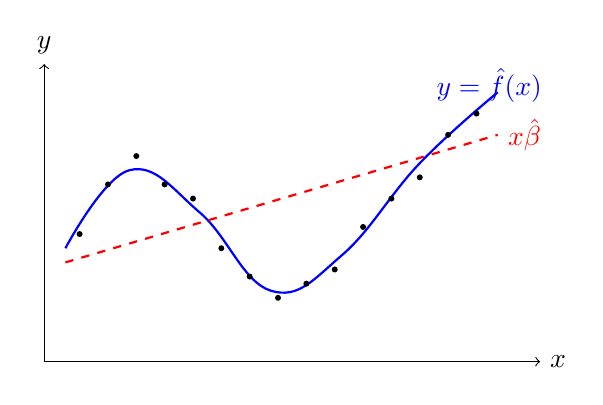
\begin{tikzpicture}[scale=0.9]
\draw[->] (0,0) -- (7,0) node[right] {$x$};
\draw[->] (0,0) -- (0,4.2) node[above] {$y$};
\draw[blue,thick] plot[smooth,tension=0.7] coordinates {(0.3,1.6) (1.2,2.7) (2.2,2.1) (3.2,1.0) (4.2,1.5) (5.3,2.8) (6.4,3.8)};
\node[blue,right] at (5.4,3.9) {$y=\hat f(x)$};
\draw[red,dashed,thick] (0.3,1.4) -- (6.4,3.2) node[right] {$x\T\hat\beta$};
\foreach \p in {(0.5,1.8),(0.9,2.5),(1.3,2.9),(1.7,2.5),(2.1,2.3),(2.5,1.6),(2.9,1.2),(3.3,0.9),(3.7,1.1),(4.1,1.3),(4.5,1.9),(4.9,2.3),(5.3,2.6),(5.7,3.2),(6.1,3.5)} \fill \p circle (1.2pt);
\end{tikzpicture}
\captionof{figure}{非参数拟合 $\hat f(x)$（实线，可任意弯曲）与线性拟合（虚线）}\label{fig:U02-np}
\end{center}

\begin{english}
A nonparametric model $y_i=f(x_i)+u_i$ is flexible but computationally demanding and suffers from the curse of dimensionality; $f$ can be estimated by kernel or series (sieve) methods. The linear model $y_i=x_i'\beta+u_i$ imposes a functional form, but it is easy to estimate and its coefficients have direct interpretations as marginal effects. Even when $f$ is nonlinear, the linear model delivers the best linear approximation to it.
\end{english}

\begin{prac}[模型分类]
判断下列模型属于参数模型还是非参数模型：(a) $y=\beta_0+\beta_1x+\beta_2x^2+u$；(b) $y=f(x)+u$，$f$ 仅假设二阶可导；(c) $y=\sum_{j=0}^{J_n}\gamma_jx^j+u$，$J_n\to\infty$。
\answer
(a) 参数模型：只有 3 个未知参数，且对参数线性（含 $x^2$ 不影响）。(b) 非参数模型：未知的是整个函数。(c) 形式上是多项式回归，但项数 $J_n$ 随样本量增长，目标是逼近未知函数 $f$，属于非参数的级数（筛）估计；对固定的 $J$ 可用 OLS 计算。
\end{prac}

%======================================================================
\section{条件期望函数与 CEF 分解}\label{sec:U02-cef}

本节是全章的基石：先定义条件期望，再用“加一项、减一项”把任意 $y$ 分解为“条件期望 $+$ 误差”，并证明这个误差的条件均值必为零。

\subsection{条件期望的定义与计算}

\subsubsection{离散与连续情形的定义}

\begin{defn}[条件期望函数 CEF]\label{def:U02-cef}
给定 $x=x_0$，$y$ 的\term{条件期望}{conditional expectation}是条件分布的均值：
\[
\E(y\mid x=x_0)=
\begin{cases}
\sum_j y_j\,P(y=y_j\mid x=x_0), & \text{离散},\\[4pt]
\int y\,f_{y\mid x}(y\mid x_0)\,\dd y,\quad f_{y\mid x}(y\mid x_0)=\dfrac{f(y,x_0)}{f_x(x_0)}, & \text{连续}.
\end{cases}
\]
把 $x_0$ 看作变量，得到函数 $m(x)=\E(y\mid x)$，称为\term{条件期望函数}{conditional expectation function, CEF}，也叫\term{回归函数}{regression function}。
\end{defn}

\subsubsection{\texorpdfstring{$m(x)$}{m(x)} 是函数，\texorpdfstring{$\E(y_i\mid x_i)$}{E(y\_i|x\_i)} 是随机变量}

对固定的 $x_0$，$\E(y\mid x=x_0)=m(x_0)$ 是一个数；把 $x$ 换成随机变量 $x_i$，$\E(y_i\mid x_i)=m(x_i)$ 是 $x_i$ 的函数，因而本身是一个\key{随机变量}。正因为它是随机变量，才能“对它再取期望”（第 \ref{sec:U02-lie} 节）。

\subsubsection{一般定义：只需 \texorpdfstring{$\E|y|<\infty$}{E|y| < infinity}}

\tagext\ 上面的公式要求有概率质量函数或联合密度。一般情形（Hansen §2.31）：若 $\E|y|<\infty$，则存在（几乎处处唯一的）函数 $m(\cdot)$，使对一切集合 $\mathcal A$ 有
\[
\E\big[\mathbf{1}\{x\in\mathcal A\}\,y\big]=\E\big[\mathbf{1}\{x\in\mathcal A\}\,m(x)\big].
\]
有联合密度时，这个 $m(\cdot)$ 就是上面的积分公式。因此本章各结论的最低条件都是 $\E|y|<\infty$。

\subsubsection{例：离散联合分布（贯穿本章的例子）}

\begin{exmp}[离散联合分布：贯穿本章的例子]\label{ex:U02-disc}
设 $x\in\{0,1,2\}$，$y\in\{0,2\}$，联合分布为
\begin{center}
\begin{tabular}{cccc}
\toprule
 & $x=0$ & $x=1$ & $x=2$\\
\midrule
$y=0$ & $1/6$ & $1/3$ & $1/6$\\
$y=2$ & $1/6$ & $0$ & $1/6$\\
\bottomrule
\end{tabular}
\end{center}
求条件期望函数 $m(x)$。
\solution
边际分布：每列相加，$P(x=0)=P(x=1)=P(x=2)=1/3$。以 $x=0$ 为例：
\begin{align*}
\E(y\mid x=0)&=0\cdot P(y=0\mid x=0)+2\cdot P(y=2\mid x=0) \why{离散条件期望定义}\\
&=2\cdot\frac{P(y=2,x=0)}{P(x=0)} \why{条件概率 $=$ 联合/边际}\\
&=2\cdot\frac{1/6}{1/3}=1. \why{查表}
\end{align*}
同理 $\E(y\mid x=1)=2\cdot\frac{0}{1/3}=0$，$\E(y\mid x=2)=2\cdot\frac{1/6}{1/3}=1$。所以 CEF 呈 U 形：
\[
m(0)=1,\qquad m(1)=0,\qquad m(2)=1.
\]
后文用这个例子说明迭代期望律、最优预测、条件方差和线性投影。
\end{exmp}

\subsection{CEF 分解：加一项、减一项}

\subsubsection{构造：加减同一项}

对任意满足 $\E|y_i|<\infty$ 的 $(y_i,x_i)$，在 $y_i$ 上加、减同一项 $\E(y_i\mid x_i)$：
\begin{align*}
y_i&=y_i+\E(y_i\mid x_i)-\E(y_i\mid x_i) \why{加减同一项，恒等式}\\
&=\E(y_i\mid x_i)+\underbrace{\big[y_i-\E(y_i\mid x_i)\big]}_{\equiv\,u_i} \why{把 $y_i$ 与 $-\E(y_i\mid x_i)$ 合并}\\
&=\E(y_i\mid x_i)+u_i,\qquad u_i\equiv y_i-\E(y_i\mid x_i). \why{定义 CEF 误差}
\end{align*}
$u_i$ 称为 \term{CEF 误差}{CEF error}，这一分解称为 \term{CEF 分解}{CEF decomposition}。

\subsubsection{分解对任何联合分布都成立}

上面每一步都是恒等变形，没有用到任何模型假设，所以 CEF 分解对\key{任何}联合分布都成立——这是它的威力所在：任何 $y$ 都可以写成“$x$ 能解释的部分 $m(x)$”加“$x$ 不能解释的部分 $u$”。

\subsection{CEF 误差的条件均值为零}

\subsubsection{结论与一行证明}

\begin{thm}[CEF 误差的条件均值为零]\label{thm:U02-meanzero}
若 $\E|y_i|<\infty$，则 $u_i=y_i-\E(y_i\mid x_i)$ 满足 $\E(u_i\mid x_i)=0$。
\end{thm}

思路：对 $u_i$ 的定义式取条件期望，利用“$\E(y_i\mid x_i)$ 是 $x_i$ 的函数，给定 $x_i$ 时是常数”。
\begin{align*}
\E(u_i\mid x_i)&=\E\big[y_i-\E(y_i\mid x_i)\,\big|\,x_i\big] \why{代入 $u_i$ 的定义}\\
&=\E(y_i\mid x_i)-\E\big[\E(y_i\mid x_i)\,\big|\,x_i\big] \why{条件期望的线性性}\\
&=\E(y_i\mid x_i)-\E(y_i\mid x_i)=0. \why{$x_i$ 的函数给定 $x_i$ 时是常数}
\end{align*}
所以在 CEF 分解中，“误差条件均值为零”是\key{定义出来的}，不是假设。$\E(u_i\mid x_i)=0$ 这一条件通常称为\term{外生性}{exogeneity}。

\subsubsection{“由构造成立”与“外生性假设”的区别}

\begin{note}[由构造成立 vs.\ 外生性假设]
若 $u$ 被定义为 CEF 误差，$\E(u\mid x)=0$ 自动成立，没有任何经济含义。但在\term{结构模型}{structural model}中，$u$ 有独立的经济含义（如“能力”），此时 $\E(u\mid x)=0$ 是一个需要论证的假设，可能不成立（第 7 章内生性）。考试中写“exogeneity”时，要分清是哪一种。
\end{note}

\begin{prac}[在离散例中直接验证 \texorpdfstring{$\E(u\mid x)=0$}{E(u|x)=0}]
在例 \ref{ex:U02-disc} 中写出 $u=y-\E(y\mid x)$ 的全部可能取值及其条件概率，并直接验证 $\E(u\mid x=0)=0$。
\answer
$x=0$ 时 $m(0)=1$：$y=0\Rightarrow u=-1$，$y=2\Rightarrow u=1$，条件概率各为 $\frac{1/6}{1/3}=\frac12$，故
\[
\E(u\mid x=0)=\tfrac12(-1)+\tfrac12(1)=0.
\]
$x=1$ 时 $m(1)=0$，$y=0$ 以条件概率 1 出现，$u=0$，$\E(u\mid x=1)=0$。$x=2$ 时与 $x=0$ 相同，$u=\pm1$ 各半，$\E(u\mid x=2)=0$。可见每个 $x$ 处 $u$ 的条件均值都为 0。
\end{prac}

\subsection{命名辨析：“projection model”与 CEF 误差分解}

\subsubsection{为何把 \texorpdfstring{$y=\E(y\mid x)+u$}{y = E(y|x) + u} 称为“projection model”}

CEF 分解 $y_i=\E(y_i\mid x_i)+u_i$ 也常被称为 \key{projection model}（投影模型），因为 $\E(y\mid x)$ 正是 $y$ 在“所有 $x$ 的函数构成的空间”上的（均方意义下的）正交投影：误差 $u$ 与 $x$ 的任何函数都正交，即 $\E[h(x)u]=0$（第 \ref{sec:U02-err} 节性质 4）。

\subsubsection{Hansen 的用词：projection 专指最佳线性预测}

Hansen 把 $y=\E(y\mid x)+u$ 称为 \key{CEF error decomposition}，而把“projection”一词专门留给最佳线性预测——在“$x$ 的\key{线性}函数构成的空间”上的投影（第 \ref{sec:U02-blp} 节）。同一个词在不同文献中所指的空间不同，读题时看清上下文。

\subsubsection{另一种写法：误差记作 \texorpdfstring{$v_i$}{v\_i}，真值记作 \texorpdfstring{$\beta_0$}{beta\_0}}

另一种常见写法是
\[
y_i=\E(y_i\mid x_i)+v_i,\qquad v_i=y_i-\E(y_i\mid x_i),\qquad \E(v_i)=0,
\]
CEF 线性时再写成 $y_i=x_i\T\beta_0+v_i$，下标 0 表示真值。注意 $\E(v_i)=0$ 由 $\E(v_i\mid x_i)=0$ 经迭代期望律得到（第 \ref{sec:U02-err} 节性质 2），是比条件均值为零更弱的结论。

\subsection{线性 CEF 时的模型：linear projection / reduced form}

\subsubsection{代入线性 CEF 得到线性回归模型}

若 CEF 恰好是线性的，$\E(y_i\mid x_i)=x_i\T\beta$，代入 CEF 分解即得
\[
y_i=x_i\T\beta+u_i,\qquad \E(u_i\mid x_i)=0.
\]
这就是带外生误差的线性回归模型。此时线性投影（第 \ref{sec:U02-blp} 节）与 CEF 重合，所以这个模型也被称为 \key{linear projection}。

\subsubsection{“简约式”一词的含义}

这个模型也被称为\term{简约式}{reduced form}：该词强调它只描述 $y$ 与 $x$ 的统计关系，不必是结构（因果）方程（详见第 \ref{sec:U02-blp} 节末“projection model / reduced form 的含义”一小节）。

\begin{english}
For any random pair $(y,x)$ with $E|y|<\infty$ we can write $y=E(y\mid x)+u$ with $u\equiv y-E(y\mid x)$. Then $E(u\mid x)=E(y\mid x)-E(y\mid x)=0$ by construction, so this zero conditional mean is not an assumption. If the CEF is linear, $E(y\mid x)=x'\beta$, this gives the linear regression model $y=x'\beta+u$ with $E(u\mid x)=0$. In a structural model, by contrast, $E(u\mid x)=0$ is a substantive exogeneity assumption.
\end{english}

%======================================================================
\section{迭代期望定律}\label{sec:U02-lie}

\term{迭代期望定律}{law of iterated expectations, LIE}是全书使用最频繁的工具：几乎所有“由条件矩推出无条件矩”的步骤都靠它。本节给出简单形式、一般形式和条件化定理。

\subsection{简单迭代期望定律}

\subsubsection{定理与直觉}

\begin{thm}[简单迭代期望定律]\label{thm:U02-lie}
若 $\E|y|<\infty$，则
\[
\E\big[\E(y\mid x)\big]=\E(y).
\]
\end{thm}

直觉：先在每个 $x$ 组内求平均，再按各组所占比例对组均值加权平均，结果等于总平均。

\subsubsection{离散情形的证明}

设 $x$ 取值 $\{x_k\}$，$y$ 取值 $\{y_j\}$。
\begin{align*}
\E\big[\E(y\mid x)\big]&=\sum_k\E(y\mid x=x_k)\,P(x=x_k) \why{对 $x$ 的分布取期望}\\
&=\sum_k\sum_jy_j\,P(y=y_j\mid x=x_k)\,P(x=x_k) \why{条件期望定义}\\
&=\sum_k\sum_jy_j\,P(y=y_j,\,x=x_k) \why{条件概率 $\times$ 边际 $=$ 联合}\\
&=\sum_jy_j\sum_kP(y=y_j,\,x=x_k) \why{交换求和次序}\\
&=\sum_jy_j\,P(y=y_j)=\E(y). \why{对 $x$ 求和得边际}
\end{align*}

\subsubsection{例：在离散例中验证 LIE}

\begin{exmp}[离散例续：验证 LIE]\label{ex:U02-lie}
在例 \ref{ex:U02-disc} 中分别计算 $\E[\E(y\mid x)]$ 与 $\E(y)$。
\solution
\begin{align*}
\E\big[\E(y\mid x)\big]&=\tfrac13 m(0)+\tfrac13 m(1)+\tfrac13 m(2) \why{$x$ 三个值各概率 $1/3$}\\
&=\tfrac13(1+0+1)=\tfrac23. \why{代入 $m(\cdot)$}
\end{align*}
直接计算：$P(y=2)=\frac16+0+\frac16=\frac13$，故 $\E(y)=2\cdot\frac13=\frac23$。两者一致。
\end{exmp}

\subsection{一般迭代期望定律：“小信息集说了算”}

\subsubsection{定理}

\begin{thm}[一般迭代期望定律]\label{thm:U02-lie-gen}
若 $\E|y|<\infty$，则对任意随机向量 $x_1,x_2$：
\[
\E\big[\E(y\mid x_1,x_2)\,\big|\,x_1\big]=\E(y\mid x_1).
\]
\end{thm}

口诀：\key{先用大信息集求期望、再用小信息集求期望，结果等于直接用小信息集求期望}（the smaller information set wins）。简单 LIE 是 $x_1$ 为常数（没有信息）时的特例。

\subsubsection{多层嵌套的化简}

反复使用一般 LIE 可以处理多层嵌套，例如三层嵌套：
\begin{align*}
\E\Big[\E\big[\E(y\mid x_1,x_2,x_3)\mid x_1,x_2\big]\,\Big|\,x_1\Big]
&=\E\big[\E(y\mid x_1,x_2)\,\big|\,x_1\big] \why{内层 LIE：$\{x_1,x_2\}\subset\{x_1,x_2,x_3\}$}\\
&=\E(y\mid x_1). \why{再用一次 LIE}
\end{align*}
再取一次无条件期望就得到 $\E(y)$。

\subsubsection{顺序颠倒时：\texorpdfstring{$\E[\E(y\mid x_1)\mid x_1,x_2]=\E(y\mid x_1)$}{E[E(y|x1)|x1,x2] = E(y|x1)}}

\begin{note}[顺序不能反]
若先用小信息集、再用大信息集：
\[
\E\big[\E(y\mid x_1)\,\big|\,x_1,x_2\big]=\E(y\mid x_1),
\]
因为 $\E(y\mid x_1)$ 是 $x_1$ 的函数，给定 $(x_1,x_2)$ 时是已知常数，可直接提出。结果\key{不是} $\E(y\mid x_1,x_2)$。两种顺序的结果都是 $\E(y\mid x_1)$——小信息集总是胜出。
\end{note}

\subsection{条件化定理：“已知的可以提出来”}

\subsubsection{定理}

\term{条件化定理}{conditioning theorem}处理“条件期望里含有 $x$ 的函数”的情形。

\begin{thm}[条件化定理]\label{thm:U02-cond}
若 $\E|y|<\infty$，则对任意函数 $g(\cdot)$，只要 $\E|g(x)y|<\infty$，就有
\[
\E\big[g(x)y\mid x\big]=g(x)\,\E(y\mid x),\qquad
\E\big[g(x)y\big]=\E\big[g(x)\,\E(y\mid x)\big].
\]
\end{thm}

\subsubsection{两式的来源}

第一式：给定 $x$ 时 $g(x)$ 是常数，可提到期望外。第二式由第一式与简单 LIE 得到：
\begin{align*}
\E\big[g(x)y\big]&=\E\Big[\E\big[g(x)y\mid x\big]\Big] \why{简单 LIE}\\
&=\E\big[g(x)\,\E(y\mid x)\big]. \why{第一式}
\end{align*}
第二式的用处：把含 $y$ 的期望换成只含 $x$ 的期望，$y$ 只通过 $m(x)$ 出现。

\subsubsection{例：线性 CEF 下计算 \texorpdfstring{$\E(xy)$}{E(xy)}}

\begin{exmp}[线性 CEF 下计算 \texorpdfstring{$\E(xy)$}{E(xy)}]
若 $\E(y\mid x)=a+bx$，用 $x$ 的矩表示 $\E(xy)$。
\solution
\begin{align*}
\E(xy)&=\E\big[x\,\E(y\mid x)\big] \why{条件化定理，$g(x)=x$}\\
&=\E\big[x(a+bx)\big] \why{代入线性 CEF}\\
&=a\,\E(x)+b\,\E(x^2). \why{期望的线性性}
\end{align*}
\end{exmp}

\begin{english}
The law of iterated expectations states $E[E(y\mid x)]=E(y)$ and, more generally, $E[E(y\mid x_1,x_2)\mid x_1]=E(y\mid x_1)$: the smaller information set dominates. The conditioning theorem states $E[g(x)y\mid x]=g(x)E(y\mid x)$, and hence $E[g(x)y]=E[g(x)E(y\mid x)]$.
\end{english}

\begin{prac}[用 LIE 与条件化定理计算条件矩]
设 $\E(y\mid x_1,x_2)=1+2x_1+3x_2$，$\E(x_2\mid x_1)=x_1^2$。求 $\E(y\mid x_1)$ 与 $\E(x_1y)$（用 $x_1$ 的矩表示）。
\answer
\begin{align*}
\E(y\mid x_1)&=\E\big[\E(y\mid x_1,x_2)\,\big|\,x_1\big] \why{一般 LIE}\\
&=\E\big[1+2x_1+3x_2\,\big|\,x_1\big] \why{代入}\\
&=1+2x_1+3\,\E(x_2\mid x_1) \why{线性性，提出 $x_1$}\\
&=1+2x_1+3x_1^2. \why{已知 $\E(x_2\mid x_1)$}
\end{align*}
再由条件化定理：
\begin{align*}
\E(x_1y)&=\E\big[x_1\,\E(y\mid x_1)\big] \why{条件化定理}\\
&=\E\big[x_1(1+2x_1+3x_1^2)\big]=\E(x_1)+2\E(x_1^2)+3\E(x_1^3). \why{期望的线性性}
\end{align*}
\end{prac}

%======================================================================
\section{CEF 误差的性质}\label{sec:U02-err}

CEF 误差 $u=y-\E(y\mid x)$ 除了条件均值为零，还有一组由它推出的性质。其中“与 $x$ 的任何函数都不相关”是后面最优预测、方差分解、线性投影等结论的共同钥匙。

\subsection{四条基本性质}

\begin{thm}[CEF 误差的性质（Hansen §2.8）]\label{thm:U02-errprop}
设 $\E|y|<\infty$，$u=y-\E(y\mid x)$。则
\begin{enumerate}[label=\arabic*.]
  \item $\E(u\mid x)=0$；
  \item $\E(u)=0$；
  \item 若 $\E|y|^r<\infty$（$r\ge1$），则 $\E|u|^r<\infty$（矩的存在性传递给误差）；
  \item 对任意函数 $h(\cdot)$，只要 $\E|h(x)u|<\infty$，就有 $\E[h(x)u]=0$。
\end{enumerate}
\end{thm}

\subsection{性质的证明}

\subsubsection{性质 1：条件均值为零}

见结论 \ref{thm:U02-meanzero}。

\subsubsection{性质 2：无条件均值为零}

\begin{align*}
\E(u)&=\E\big[\E(u\mid x)\big] \why{简单 LIE}\\
&=\E[0]=0. \why{性质 1}
\end{align*}

\subsubsection{性质 3：矩的存在性由 \texorpdfstring{$y$}{y} 传给 \texorpdfstring{$u$}{u}}

记 $m(x)=\E(y\mid x)$。先证 $m(x)$ 的 $r$ 阶矩不超过 $y$ 的，再用 Minkowski 不等式。
\begin{align*}
\E|m(x)|^r&=\E\big|\E(y\mid x)\big|^r \why{$m$ 的定义}\\
&\le\E\big[\E(|y|^r\mid x)\big] \why{条件 Jensen：$|\cdot|^r$ 凸}\\
&=\E|y|^r<\infty, \why{简单 LIE}\\
\big(\E|u|^r\big)^{1/r}&=\big(\E|y-m(x)|^r\big)^{1/r} \why{$u$ 的定义}\\
&\le\big(\E|y|^r\big)^{1/r}+\big(\E|m(x)|^r\big)^{1/r} \why{Minkowski 不等式}\\
&\le2\big(\E|y|^r\big)^{1/r}<\infty. \why{上一段结论}
\end{align*}
常用特例：$r=2$，即 $\E y^2<\infty\Rightarrow\E u^2<\infty$。

\subsubsection{性质 4：\texorpdfstring{$\E[h(x)u]=0$}{E[h(x)u] = 0}}

思路：先对 $x$ 取条件期望，把 $h(x)$ 当常数提出。
\begin{align*}
\E\big[h(x)u\big]&=\E\Big[\E\big(h(x)u\mid x\big)\Big] \why{简单 LIE}\\
&=\E\big[h(x)\,\E(u\mid x)\big] \why{条件化定理：$h(x)$ 给定 $x$ 时为常数}\\
&=\E\big[h(x)\cdot0\big]=0. \why{性质 1}
\end{align*}

\subsection{误差与 \texorpdfstring{$x$}{x} 的任何函数都不相关}

\subsubsection{取 \texorpdfstring{$h(x)=x$}{h(x)=x}：\texorpdfstring{$\E(xu)=0$}{E(xu)=0} 与 \texorpdfstring{$\Cov(x,u)=0$}{Cov(x,u)=0}}

\begin{align*}
\Cov(x,u)&=\E(xu)-\E(x)\E(u) \why{协方差定义}\\
&=\E(xu) \why{性质 2：$\E u=0$}\\
&=0. \why{性质 4，$h(x)=x$}
\end{align*}

\subsubsection{取 \texorpdfstring{$h(x)=x^2,\ \log x,\ \mathbf{1}\{x>0\}$}{h(x) = x\^2, log x, 1\{x>0\}}：同样不相关}

性质 4 对任何（可积的）$h$ 都成立，所以 $\E(x^2u)=0$、$\E(u\log x)=0$、$\E(u\,\mathbf{1}\{x>0\})=0$ 等都对。结论：\key{CEF 误差与 $x$ 的任何（可积）函数都不相关}。例如判断题“若 $\E(e\mid X)=0$，则 $\E(X^2e)=0$”是对的（取 $h(x)=x^2$）。

\subsection{均值独立、不相关与独立的强弱关系}

\subsubsection{强弱链条}

三个常被混淆的概念由强到弱为：
\[
\underbrace{u\indep x}_{\text{独立}}
\ \Longrightarrow\ 
\underbrace{\E(u\mid x)=0}_{\text{均值独立（设 }\E u=0\text{）}}
\ \Longrightarrow\ 
\underbrace{\E(xu)=0,\ \E u=0}_{\text{不相关}}.
\]
第一个箭头：独立时条件分布等于边际分布，$\E(u\mid x)=\E(u)=0$。第二个箭头：性质 2 与性质 4（$h(x)=x$）。反向均不成立，下面给出反例。

\subsubsection{反例一：均值独立推不出独立}

设 $u\mid x\sim N(0,x^2)$。则 $\E(u\mid x)=0$，但 $u$ 的条件方差 $x^2$ 依赖 $x$，所以 $u$ 与 $x$ 不独立。因此“$\E(u\mid x)=0\Rightarrow u$ 与 $x$ 独立”是错的。

即使再加上同方差 $\E(u^2\mid x)=\sigma^2$，也推不出独立：例如 $x\in\{0,1\}$，$x=0$ 时 $u\sim N(0,1)$，$x=1$ 时 $u$ 以各 $1/2$ 的概率取 $\pm1$。两种情形下条件均值都是 0、条件方差都是 1，但条件分布不同（四阶矩分别为 3 与 1），故不独立。一般地，三阶、四阶等更高阶矩仍可依赖 $x$。

\subsubsection{反例二：不相关推不出均值独立}

设 $x\sim N(0,1)$，$u=x^2-1$。
\begin{align*}
\E(u)&=\E(x^2)-1=1-1=0, \why{$\E x^2=1$}\\
\E(xu)&=\E(x^3)-\E(x)=0-0=0, \why{标准正态奇数阶矩为 0}\\
\E(u\mid x)&=x^2-1\neq0. \why{$u$ 是 $x$ 的函数}
\end{align*}
所以 $u$ 与 $x$ 不相关，却不均值独立。同一例子还说明 $\E(xu)=0$ 推不出 $\E(x^2u)=0$：
\begin{align*}
\E(x^2u)&=\E(x^4)-\E(x^2) \why{代入 $u=x^2-1$}\\
&=3-1=2\neq0. \why{$\E x^4=3$}
\end{align*}

\subsection{只含截距的模型与回归方差}

\subsubsection{只含截距的模型}

若没有任何回归元，“条件期望”退化为无条件期望，CEF 分解成为\term{只含截距的模型}{intercept-only model}：
\[
y=\mu+u,\qquad \mu=\E(y),\qquad \E(u)=0.
\]

\subsubsection{回归方差 \texorpdfstring{$\sigma^2=\E(u^2)$}{sigma\^2 = E(u\^2)}}

\term{回归方差}{regression variance}定义为 CEF 误差的方差：
\[
\sigma^2=\Var(u)=\E(u^2)\qquad(\text{因 }\E u=0).
\]
由性质 3（$r=2$），若 $\E y^2<\infty$ 则 $\sigma^2<\infty$。$\sigma^2$ 度量 $y$ 中不能被 $x$ 解释的变异。

\subsubsection{方差分解 \texorpdfstring{$\Var(y)=\Var(m(x))+\sigma^2$}{Var(y) = Var(m(x)) + sigma\^2}}

思路：$y=m(x)+u$ 的两部分不相关，所以方差可加。
\begin{align*}
\Cov\big(m(x),u\big)&=\E\big[m(x)u\big]-\E\big[m(x)\big]\E(u) \why{协方差定义}\\
&=\E\big[m(x)u\big]=0, \why{性质 2 与性质 4，$h=m$}\\
\Var(y)&=\Var\big(m(x)+u\big) \why{CEF 分解}\\
&=\Var\big(m(x)\big)+\Var(u)+2\Cov\big(m(x),u\big) \why{和的方差}\\
&=\Var\big(m(x)\big)+\sigma^2. \why{协方差为 0}
\end{align*}
即：总方差 $=$ $x$ 能解释的方差 $+$ 回归方差。由此 $\sigma^2\le\Var(y)$，这是第 \ref{sec:U02-var} 节全方差公式的前一半。

\begin{english}
The CEF error satisfies $E(u\mid x)=0$, $E(u)=0$, and $E[h(x)u]=0$ for any function $h$ (proof: by the law of iterated expectations, $E[h(x)u]=E[h(x)E(u\mid x)]=0$). Hence $u$ is uncorrelated with any function of $x$, but it need not be independent of $x$. Independence implies mean independence, which implies zero correlation; the converses fail. The regression variance is $\sigma^2=E(u^2)$, and $\mathrm{Var}(y)=\mathrm{Var}(m(x))+\sigma^2$.
\end{english}

\begin{prac}[True or False：不相关与均值独立]
(a) If $\E(u\mid x)=0$ then $\Cov(x^3,u)=0$. (b) If $\Cov(x,u)=0$ and $\E u=0$, then $\E(u\mid x)=0$.
\answer
(a) True。由性质 4 取 $h(x)=x^3$ 得 $\E(x^3u)=0$，又 $\E u=0$，故 $\Cov(x^3,u)=\E(x^3u)-\E(x^3)\E(u)=0$。

(b) False。反例 $x\sim N(0,1)$，$u=x^2-1$：$\E u=0$，$\Cov(x,u)=\E(x^3)-0=0$，但 $\E(u\mid x)=x^2-1\neq0$。
\end{prac}

%======================================================================
\section{CEF 是均方误差意义下的最优预测}\label{sec:U02-pred}

本节说明为什么 CEF 是回归分析的核心对象：在所有用 $x$ 构造的预测中，它的均方误差最小。

\subsection{预测问题与均方误差准则}

用 $x$ 的某个函数 $g(x)$ 去预测 $y$，预测误差为 $y-g(x)$。以\term{均方误差}{mean squared error, MSE}
\[
\E\big[(y-g(x))^2\big]
\]
为损失。问题：在所有函数 $g$ 中，哪个最好？

\subsection{条件均值是最优预测}

\subsubsection{定理}

\begin{thm}[条件均值是最优预测（Hansen §2.11）]\label{thm:U02-bestpred}
若 $\E y^2<\infty$，则对任意预测函数 $g(x)$，
\[
\E\big[(y-g(x))^2\big]\ \ge\ \E\big[(y-m(x))^2\big],\qquad m(x)=\E(y\mid x),
\]
等号当且仅当 $g(x)=m(x)$（几乎处处）。
\end{thm}

\subsubsection{证明：交叉项因 \texorpdfstring{$\E[h(x)u]=0$}{E[h(x)u]=0} 而消失}

思路：把 $y-g(x)$ 拆成“CEF 误差 $+$ 预测偏离”，交叉项因性质 4 而消失。
\begin{align*}
\E\big[(y-g(x))^2\big]&=\E\big[(u+m(x)-g(x))^2\big] \why{代入 $y=m(x)+u$}\\
&=\E(u^2)+2\,\E\big[u\,(m(x)-g(x))\big]+\E\big[(m(x)-g(x))^2\big] \why{展开平方}\\
&=\E(u^2)+\E\big[(m(x)-g(x))^2\big] \why{性质 4，$h(x)=m(x)-g(x)$}\\
&\ge\E(u^2)=\E\big[(y-m(x))^2\big]. \why{平方项非负}
\end{align*}
等号成立当且仅当 $\E[(m(x)-g(x))^2]=0$，即 $g(x)=m(x)$ 几乎处处。含义：在所有 $x$ 的函数中，CEF 的预测误差最小；任何其他预测都要额外付出 $\E[(m(x)-g(x))^2]$。

\subsubsection{特例：不用 \texorpdfstring{$x$}{x} 时，最优常数预测是 \texorpdfstring{$\E(y)$}{E(y)}}

若不允许用 $x$（$g$ 只能是常数），相当于条件变量没有信息，CEF 退化为 $\E(y)$，所以最优常数预测是 $\E(y)$，最小 MSE 为 $\Var(y)$（另一种推导见本章第 \ref{sec:U02-blp} 节末的即时练习）。

\subsubsection{例：离散例中 CEF 预测与常数预测的 MSE}

\begin{exmp}[离散例续：两种预测的 MSE]\label{ex:U02-mse}
在例 \ref{ex:U02-disc} 中，比较用 CEF $m(x)$ 预测与只用常数 $\E y$ 预测的 MSE。
\solution
CEF 预测的 MSE 是 $\E(u^2)$。由即时练习（第 \ref{sec:U02-cef} 节）的 $u$ 的分布：$x=0$ 或 $x=2$ 时 $u=\pm1$，$u^2=1$；$x=1$ 时 $u=0$。故
\[
\E(u^2)=\tfrac13\cdot1+\tfrac13\cdot0+\tfrac13\cdot1=\tfrac23.
\]
常数预测用 $\E y=\frac23$，其 MSE 为 $\Var(y)$：
\begin{align*}
\E(y^2)&=4\cdot P(y=2)=4\cdot\tfrac13=\tfrac43, \why{$y^2\in\{0,4\}$}\\
\Var(y)&=\E(y^2)-(\E y)^2=\tfrac43-\tfrac49=\tfrac89. \why{简便公式}
\end{align*}
$\frac89>\frac23$：利用 $x$ 的信息使 MSE 下降了 $\frac29$，这正是 $\Var(m(x))$（见例 \ref{ex:U02-vardec}）。
\end{exmp}

\subsection{信息越多，预测误差方差越小}

\subsubsection{结论}

\begin{thm}[条件变量越多，CEF 误差方差越小（Hansen §2.10）]\label{thm:U02-moreinfo}
若 $\E y^2<\infty$，则
\[
\Var(y)\ \ge\ \Var\big(y-\E(y\mid x_1)\big)\ \ge\ \Var\big(y-\E(y\mid x_1,x_2)\big).
\]
\end{thm}

\subsubsection{证明：差值是条件变量的函数，与误差正交}

记 $u_1=y-\E(y\mid x_1)$，$u_2=y-\E(y\mid x_1,x_2)$，二者均值为 0，故 $\Var(u_j)=\E(u_j^2)$。令 $d=\E(y\mid x_1,x_2)-\E(y\mid x_1)$，它是 $(x_1,x_2)$ 的函数。
\begin{align*}
u_1&=u_2+d \why{加减 $\E(y\mid x_1,x_2)$}\\
\E(u_1^2)&=\E(u_2^2)+2\,\E(d\,u_2)+\E(d^2) \why{展开平方}\\
&=\E(u_2^2)+\E(d^2) \why{性质 4：$d$ 是 $(x_1,x_2)$ 的函数}\\
&\ge\E(u_2^2). \why{$\E(d^2)\ge0$}
\end{align*}
第一个不等号用同样的论证：把“不用任何信息”的预测 $\E(y)$ 看作最小的信息集，$y-\E(y)=u_1+[\E(y\mid x_1)-\E(y)]$，后一项是 $x_1$ 的函数，与 $u_1$ 正交，故 $\Var(y)=\E(u_1^2)+\Var(\E(y\mid x_1))\ge\E(u_1^2)$。

\subsubsection{预测意义上更好不等于因果意义上更好}

\begin{note}[“多控制变量”的两种含义]
条件变量越多，CEF 误差的方差越小（至少不增）。这为“控制更多变量”提供了\key{预测}意义上的理由，但不代表\key{因果}意义上更好：控制变量是否恰当，要看它能否使条件独立假设成立（第 \ref{sec:U02-causal} 节）。
\end{note}

\begin{english}
The conditional mean $m(x)=E(y\mid x)$ is the best predictor of $y$ given $x$ in the mean-squared-error sense: for any $g(x)$, $E[(y-g(x))^2]=E(u^2)+E[(m(x)-g(x))^2]\ge E(u^2)$, because the cross term vanishes by $E[h(x)u]=0$. Conditioning on more variables (weakly) reduces the variance of the CEF error.
\end{english}

\begin{prac}[\texorpdfstring{$\sigma^2(x)$}{sigma\^2(x)} 是 \texorpdfstring{$u^2$}{u\^2} 的最优预测]
证明 $\sigma^2(x)=\E(u^2\mid x)$ 是 $u^2$ 关于 $x$ 的最优（MSE）预测。
\answer
把结论 \ref{thm:U02-bestpred} 中的 $y$ 换成 $w=u^2$。该定理对任何满足 $\E w^2<\infty$ 的随机变量成立，这里要求 $\E u^4<\infty$；其结论是 $w$ 关于 $x$ 的最优预测为 $\E(w\mid x)$。此处 $\E(u^2\mid x)=\sigma^2(x)$，所以对任意 $h(x)$，
\[
\E\big[(u^2-h(x))^2\big]\ge\E\big[(u^2-\sigma^2(x))^2\big].
\]
“预测 $u^2$”的含义是：预测给定 $x$ 时误差的大小（波动程度），这正是异方差建模的对象（第 \ref{sec:U02-var} 节）。
\end{prac}

%======================================================================
\section{条件方差、同方差与异方差}\label{sec:U02-var}

条件期望描述给定 $x$ 时 $y$ 的“中心”，条件方差描述给定 $x$ 时 $y$ 的“离散程度”。误差的条件方差是否依赖 $x$，决定了误差是同方差还是异方差。

\subsection{条件方差的定义与两种写法}

\subsubsection{定义}

\begin{defn}[条件方差]\label{def:U02-cvar}
\term{条件方差}{conditional variance}
\[
\sigma^2(x)=\Var(y\mid x)=\E\big[(y-\E(y\mid x))^2\,\big|\,x\big]=\E(u^2\mid x)=\Var(u\mid x).
\]
\end{defn}
最后一个等号成立是因为 $\Var(u\mid x)=\E(u^2\mid x)-[\E(u\mid x)]^2$，而 $\E(u\mid x)=0$。

\subsubsection{简便公式 \texorpdfstring{$\sigma^2(x)=\E(y^2\mid x)-[\E(y\mid x)]^2$}{sigma\^2(x) = E(y\^2|x) - [E(y|x)]\^2}}

展开平方可得另一写法，它与无条件的 $\Var y=\E y^2-(\E y)^2$ 完全平行。
\begin{align*}
\sigma^2(x)&=\E\big[y^2-2y\,m(x)+m(x)^2\,\big|\,x\big] \why{展开，$m(x)=\E(y\mid x)$}\\
&=\E(y^2\mid x)-2m(x)\,\E(y\mid x)+m(x)^2 \why{条件化定理}\\
&=\E(y^2\mid x)-2m(x)^2+m(x)^2 \why{$\E(y\mid x)=m(x)$}\\
&=\E(y^2\mid x)-\big[\E(y\mid x)\big]^2. \why{合并同类项}
\end{align*}

\subsection{方差分解公式}

\subsubsection{全方差公式}

\begin{thm}[方差分解（Hansen §2.12）]\label{thm:U02-vardec}
若 $\E y^2<\infty$，则
\[
\Var(y)=\E\big[\Var(y\mid x)\big]+\Var\big(\E(y\mid x)\big),
\]
即“组内方差的平均 $+$ 组均值的方差”。
\end{thm}

\subsubsection{证明}

\begin{align*}
\Var(y)&=\Var\big(m(x)\big)+\E(u^2) \why{第 \ref{sec:U02-err} 节方差分解}\\
&=\Var\big(m(x)\big)+\E\big[\E(u^2\mid x)\big] \why{简单 LIE}\\
&=\Var\big(\E(y\mid x)\big)+\E\big[\Var(y\mid x)\big]. \why{$\E(u^2\mid x)=\sigma^2(x)$}
\end{align*}

\subsubsection{例：离散例中验证方差分解}

\begin{exmp}[离散例续：条件方差与方差分解]\label{ex:U02-vardec}
在例 \ref{ex:U02-disc} 中求 $\sigma^2(x)$，并验证方差分解。
\solution
$x=0$：$\E(y^2\mid x=0)=4\cdot\frac12=2$，故 $\sigma^2(0)=2-1^2=1$。$x=1$：$y\equiv0$，$\sigma^2(1)=0$。$x=2$：同 $x=0$，$\sigma^2(2)=1$。于是
\begin{align*}
\E\big[\Var(y\mid x)\big]&=\tfrac13(1+0+1)=\tfrac23, \why{对 $x$ 取平均}\\
\E\big[m(x)\big]&=\tfrac13(1+0+1)=\tfrac23, \why{$m=(1,0,1)$}\\
\E\big[m(x)^2\big]&=\tfrac13(1+0+1)=\tfrac23, \why{$m^2=(1,0,1)$}\\
\Var\big(m(x)\big)&=\tfrac23-\tfrac49=\tfrac29, \why{简便公式}\\
\E\big[\Var(y\mid x)\big]+\Var\big(m(x)\big)&=\tfrac23+\tfrac29=\tfrac89=\Var(y). \why{例 \ref{ex:U02-mse}}
\end{align*}
方差分解成立。注意 $\E[\Var(y\mid x)]=\frac23$ 正是 CEF 预测的 MSE。
\end{exmp}

\subsection{同方差与异方差}

\subsubsection{定义}

\begin{defn}[同方差与异方差]\label{def:U02-homo}
若 $\sigma^2(x)=\E(u^2\mid x)=\sigma^2$ 不依赖 $x$，称误差\term{同方差}{homoskedastic}；若 $\sigma^2(x)$ 随 $x$ 变化，称误差\term{异方差}{heteroskedastic}。
\end{defn}

\subsubsection{带下标的写法 \texorpdfstring{$\sigma_i^2$}{sigma\_i\^2}}

常见的简写是：同方差 $\E(u_i^2)=\sigma^2=\Var(u_i)$；异方差 $\E(u_i^2)=\sigma_i^2=\Var(u_i)$。下标 $i$ 表示“每个观测的方差不同”，实质是 $\sigma_i^2=\sigma^2(x_i)$。严格写法应以 $x_i$ 为条件：$\E(u_i^2\mid x_i)=\sigma^2$ 或 $\sigma^2(x_i)$。

\subsubsection{易错点}

\begin{note}[同方差的三个易错点]
\begin{itemize}
  \item 同方差是关于\key{二阶矩}的假设，与 $\E(u\mid x)=0$（一阶矩）相互独立：一个成立不意味着另一个成立。
  \item 例 \ref{ex:U02-vardec} 中 $\sigma^2(0)=1$，$\sigma^2(1)=0$，$\sigma^2(2)=1$，是异方差。
  \item 在 OLS 理论中，同方差只影响方差公式与有效性（Gauss--Markov 定理），不影响无偏性和一致性（第 4、5 章）。
\end{itemize}
\end{note}

\subsection{异方差是常态：泊松模型与随机系数}

\subsubsection{例：泊松条件分布}

\begin{exmp}[泊松条件分布导出异方差的线性 CEF]
设 $y\mid x\sim\text{Poisson}(x\T\beta)$（$x\T\beta>0$）。判断线性回归是否正确设定、误差是否同方差。
\solution
泊松分布的均值与方差都等于参数，所以
\[
\E(y\mid x)=x\T\beta,\qquad \Var(y\mid x)=x\T\beta.
\]
CEF 线性，故 $y=x\T\beta+u$、$\E(u\mid x)=0$ 是正确设定的线性回归；但 $\Var(u\mid x)=\Var(y\mid x)=x\T\beta$ 随 $x$ 变化——异方差。所以线性回归可用，但标准误须用异方差稳健形式（第 5 章）。
\end{exmp}

\subsubsection{随机系数模型导出 \texorpdfstring{$\Var(u\mid x)=x\T\Sigma x$}{Var(u|x) = x' Sigma x}}

随机系数模型（第 \ref{sec:U02-causal} 节）同样导出异方差：$\Var(u\mid x)=x\T\Sigma x$。再加上 0-1 因变量（下面的即时练习）等情形，经济数据中\key{同方差是例外而非常态}。

\begin{english}
The conditional variance is $\sigma^2(x)=\mathrm{Var}(y\mid x)=E(u^2\mid x)=E(y^2\mid x)-[E(y\mid x)]^2$, and $\mathrm{Var}(y)=E[\mathrm{Var}(y\mid x)]+\mathrm{Var}(E(y\mid x))$. The error is homoskedastic if $\sigma^2(x)=\sigma^2$ does not depend on $x$, and heteroskedastic otherwise. Homoskedasticity is a second-moment condition and is not implied by $E(u\mid x)=0$.
\end{english}

\begin{prac}[二值变量的条件均值与条件方差]
设 $x,y\in\{0,1\}$，$P(x=0,y=0)=0.2$，$P(x=0,y=1)=0.3$，$P(x=1,y=0)=0.4$，$P(x=1,y=1)=0.1$。求 $\E(y\mid x)$、$\Var(y\mid x)$，并判断是否同方差。
\answer
边际：$P(x=0)=0.2+0.3=0.5$，$P(x=1)=0.4+0.1=0.5$。
\begin{align*}
\E(y\mid x=0)&=P(y=1\mid x=0)=0.3/0.5=0.6, \why{0-1 变量的均值即概率}\\
\E(y\mid x=1)&=P(y=1\mid x=1)=0.1/0.5=0.2. \why{同上}
\end{align*}
$y$ 为 0-1 变量，$y^2=y$，所以 $\E(y^2\mid x)=\E(y\mid x)$，条件方差为 $p(1-p)$：
\begin{align*}
\Var(y\mid x=0)&=0.6-0.6^2=0.24, \why{简便公式}\\
\Var(y\mid x=1)&=0.2-0.2^2=0.16. \why{简便公式}
\end{align*}
条件方差随 $x$ 变化，是异方差。0-1 因变量的线性概率模型天然异方差。
\end{prac}

%======================================================================
\section{回归导数与系数解释}\label{sec:U02-deriv}

本节回答“$\beta_j$ 是什么意思”：它首先是回归导数（条件均值的变化率），在不同语境下又被称为边际效应、偏效应或条件因果效应；对数模型中则读作百分比变化。

\subsection{回归导数（边际效应）}

\subsubsection{定义：连续变量与虚拟变量}

\begin{defn}[回归导数]\label{def:U02-deriv}
对连续变量 $x_1$，\term{回归导数}{regression derivative}为
\[
\frac{\partial m(x)}{\partial x_1},
\]
即其他回归元不变时，$x_1$ 增加一单位，$y$ 的条件均值变化多少。对虚拟变量 $x_1\in\{0,1\}$，回归导数定义为差分 $m(1,x_2)-m(0,x_2)$。
\end{defn}

\subsubsection{线性 CEF 下系数即回归导数}

在线性 CEF $m(x)=x\T\beta=\sum_k\beta_kx_k$ 下，对 $x_j$ 求偏导只剩第 $j$ 项：
\[
\frac{\partial m(x)}{\partial x_j}=\beta_j,
\]
即系数就是回归导数，且不依赖评估点。

\subsubsection{两点提醒}

\begin{note}[回归导数的两点提醒]
(1) 它描述的是\key{条件均值}的变化，不是某个个体 $y$ 的变化；(2) “其他条件不变”只针对\key{模型中已包含}的回归元，遗漏的变量仍可能随 $x_1$ 变化（第 \ref{sec:U02-ovb} 节）。
\end{note}

\subsection{\texorpdfstring{$\beta$}{beta} 的三种解释：边际效应、偏效应、条件因果效应}

$\beta$ 常被同时称为 marginal effects / partial effects / conditional causal effects。三种说法侧重点不同：

\subsubsection{边际效应：条件均值的变化率}

\term{边际效应}{marginal effect}：$\beta_j=\partial\E(y\mid x)/\partial x_j$，$x_j$ 变动一单位时 $y$ 条件均值的变动。

\subsubsection{偏效应：保持其他回归元不变}

\term{偏效应}{partial effect}：强调“偏导数”——保持其他回归元不变（控制其他变量）。它对应第 \ref{sec:U02-ovb} 节的分块投影公式，以及第 3 章 FWL 定理中的“partialling out”（先剔除其他变量的影响，再看 $x_j$ 与 $y$ 的关系）。

\subsubsection{条件因果效应：需要条件独立假设}

\term{条件因果效应}{conditional causal effect}：在条件独立/外生性成立时（第 \ref{sec:U02-causal} 节），$\beta_j$ 可以解释为给定其他变量时 $x_j$ 对 $y$ 的（平均）因果效应。没有这个假设，$\beta_j$ 只是统计关联。“conditional”一词正是指“给定（控制）其他变量”。

\subsection{对数模型中系数的百分比解释}

\subsubsection{四种函数形式对照表}

\tagext\ 工资方程常取对数，系数的解释随之改变（答题常用）：
\begin{center}
\small
\begin{tabularx}{\linewidth}{lllL}
\toprule
模型 & $\beta_1$ 的含义 & 名称 & 近似解释\\
\midrule
$y=\beta_0+\beta_1x$ & $\Delta y/\Delta x$ & 水平—水平 & $x$ 增 1 单位，$y$ 增 $\beta_1$ 单位\\
$\log y=\beta_0+\beta_1x$ & $\Delta\log y/\Delta x$ & 半弹性 & $x$ 增 1 单位，$y$ 约增 $100\beta_1\%$\\
$y=\beta_0+\beta_1\log x$ & $\Delta y/\Delta\log x$ & --- & $x$ 增 $1\%$，$y$ 约增 $\beta_1/100$ 单位\\
$\log y=\beta_0+\beta_1\log x$ & $\Delta\log y/\Delta\log x$ & 弹性 & $x$ 增 $1\%$，$y$ 约增 $\beta_1\%$\\
\bottomrule
\end{tabularx}
\captionof{table}{对数模型中系数的解释}
\end{center}

\subsubsection{近似解释的来源：\texorpdfstring{$\Delta\log y\approx\Delta y/y$}{Delta log y ≈ Delta y / y}}

三种近似都来自小变化下的 $\Delta\log y\approx\Delta y/y$（相对变化）。以半弹性与“水平—对数”为例：
\begin{align*}
\Delta\log y&=\beta_1\Delta x \why{$\log y=\beta_0+\beta_1x$ 取差分}\\
\frac{\Delta y}{y}&\approx\beta_1\Delta x \why{$\Delta\log y\approx\Delta y/y$}\\
100\cdot\frac{\Delta y}{y}&\approx100\beta_1\quad(\Delta x=1); \why{化为百分比}\\
\Delta y&=\beta_1\Delta\log x\approx\beta_1\frac{\Delta x}{x} \why{$y=\beta_0+\beta_1\log x$}\\
&=\beta_1\times0.01=\beta_1/100\quad(\Delta x/x=1\%). \why{$x$ 增 $1\%$}
\end{align*}
弹性同理：$\Delta\log y=\beta_1\Delta\log x$，两边都换成相对变化即得。

\subsubsection{半弹性的精确值 \texorpdfstring{$100(e^{\beta_1}-1)\%$}{100(exp(beta1)-1)\%}}

$x$ 增加 1 单位时，设 $y$ 由 $y_0$ 变为 $y_1$：
\begin{align*}
\log y_1-\log y_0&=\beta_1 \why{半弹性模型，$\Delta x=1$}\\
\frac{y_1}{y_0}&=e^{\beta_1} \why{两边取指数}\\
\frac{y_1-y_0}{y_0}&=e^{\beta_1}-1. \why{两边减 1}
\end{align*}
所以精确的百分比变化是 $100(e^{\beta_1}-1)\%$。因 $e^{\beta_1}-1\approx\beta_1$（$\beta_1$ 小），$\beta_1$ 较小时（如 $|\beta_1|<0.1$）近似误差可忽略。

\begin{english}
In the linear CEF model the coefficient $\beta_j=\partial E(y\mid x)/\partial x_j$ is the regression derivative: the marginal (partial) effect of $x_j$ on the conditional mean of $y$, holding the other included regressors fixed. It can be interpreted as a (conditional) causal effect only under additional assumptions such as conditional independence. In a log-level model, $100\beta_j$ is approximately the percentage change in $y$ for a one-unit change in $x_j$; the exact change is $100(e^{\beta_j}-1)\%$.
\end{english}

\begin{prac}[含平方项的对数工资方程]
$\widehat{\log(wage)}=0.531+0.144\,educ+0.043\,exper-0.095\,exper^2/100$。求经验 $exper=10$ 时，多一年经验对工资的近似百分比影响；多一年教育呢？
\answer
对 $exper$ 求导：
\begin{align*}
\frac{\partial\widehat{\log(wage)}}{\partial\,exper}&=0.043-2\times0.095\times\frac{exper}{100} \why{平方项求导}\\
&=0.043-0.0019\times10=0.024, \why{代入 $exper=10$}
\end{align*}
即多一年经验工资约增 $2.4\%$。教育：系数 $0.144$，约增 $14.4\%$；精确值 $100(e^{0.144}-1)\%\approx15.5\%$。
\end{prac}

%======================================================================
\section{线性 CEF 模型}\label{sec:U02-lincef}

本节把“CEF 是线性的”作为假设写成模型，并说明这个假设比看上去灵活：回归元可以含平方项、交互项与虚拟变量；全是离散回归元且包含全部交互项时，线性 CEF 甚至一定成立。

\subsection{线性 CEF 模型与同方差线性 CEF 模型}

\begin{defn}[线性 CEF 模型]\label{def:U02-lincef}
\term{线性 CEF 模型}{linear CEF model}：
\[
y=x\T\beta+u,\qquad \E(u\mid x)=0.
\]
若再有 $\E(u^2\mid x)=\sigma^2$，称为\term{同方差线性 CEF 模型}{homoskedastic linear CEF model}。
\end{defn}

线性 CEF 是一个\key{假设}：真实 CEF 未必线性。但下面两种情形下它可以非常灵活。

\subsection{含非线性项的线性 CEF：平方项与交互项}

\subsubsection{“线性”指对参数线性}

回归元可以是原始变量的非线性变换。例如
\[
m(x_1,x_2)=\beta_0+\beta_1x_1+\beta_2x_2+\beta_3x_1^2+\beta_4x_2^2+\beta_5x_1x_2
\]
对 $(x_1,x_2)$ 是二次的，但对参数 $\beta$ 是线性的，只要把 $x=(1,x_1,x_2,x_1^2,x_2^2,x_1x_2)\T$ 作为回归元向量，它仍是线性 CEF 模型。

\subsubsection{边际效应依赖评估点}

此时 $x_1$ 的边际效应不再是单个系数：
\begin{align*}
\frac{\partial m}{\partial x_1}&=\beta_1+2\beta_3x_1+\beta_5x_2, \why{逐项对 $x_1$ 求偏导}
\end{align*}
依赖评估点 $(x_1,x_2)$。报告时常在样本均值处计算，或报告其样本平均（平均边际效应）。

\subsubsection{交互效应 \texorpdfstring{$\beta_5$}{beta\_5}}

再对 $x_2$ 求导：$\partial^2m/\partial x_1\partial x_2=\beta_5$。所以 $\beta_5$ 度量\term{交互效应}{interaction effect}：$x_2$ 每增加一单位，$x_1$ 的边际效应变化 $\beta_5$。

\subsection{含虚拟变量的线性 CEF}

记 $\mu_{ab}=\E(y\mid x_1=a,x_2=b)$ 为格子均值。

\subsubsection{一个虚拟变量：CEF 必为线性}

$x_1\in\{0,1\}$ 时 CEF 只取两个值 $\mu_0,\mu_1$，总可写成线性形式：
\begin{align*}
m(x_1)&=\mu_0(1-x_1)+\mu_1x_1 \why{$x_1=0$ 得 $\mu_0$，$x_1=1$ 得 $\mu_1$}\\
&=\mu_0+(\mu_1-\mu_0)x_1\equiv\beta_0+\beta_1x_1, \why{整理}
\end{align*}
$\beta_0=\mu_0$，$\beta_1=\mu_1-\mu_0$（组均值之差）。所以一个虚拟变量的 CEF \key{一定}是线性的。

\subsubsection{两个虚拟变量：需要交互项}

$x_1,x_2\in\{0,1\}$ 时 CEF 取 4 个值 $\mu_{00},\mu_{01},\mu_{10},\mu_{11}$，需要 4 个参数：
\[
m(x_1,x_2)=\beta_0+\beta_1x_1+\beta_2x_2+\beta_3x_1x_2.
\]
依次代入四个格子求参数：
\begin{align*}
\mu_{00}&=\beta_0, \why{$x_1=x_2=0$}\\
\mu_{10}&=\beta_0+\beta_1\ \Rightarrow\ \beta_1=\mu_{10}-\mu_{00}, \why{$x_1=1,x_2=0$}\\
\mu_{01}&=\beta_0+\beta_2\ \Rightarrow\ \beta_2=\mu_{01}-\mu_{00}, \why{$x_1=0,x_2=1$}\\
\mu_{11}&=\beta_0+\beta_1+\beta_2+\beta_3\ \Rightarrow\ \beta_3=(\mu_{11}-\mu_{01})-(\mu_{10}-\mu_{00}). \why{$x_1=x_2=1$}
\end{align*}
$\beta_3$ 是“$x_2=1$ 时 $x_1$ 的效应”减去“$x_2=0$ 时 $x_1$ 的效应”。若省略交互项，就隐含了约束 $\beta_3=0$，即“$x_1$ 的效应不随 $x_2$ 变化”。

\subsubsection{饱和模型：离散回归元的 CEF 总是线性的}

一般结论：当所有回归元只取有限个值，且回归中包含全部虚拟变量及其全部交互项时，参数个数等于格子个数，CEF 一定可以写成线性形式。这样的模型称为\term{饱和模型}{saturated model}。

\subsubsection{例：二值变量加三分类变量}

\begin{exmp}[二值变量 \texorpdfstring{$+$}{+} 三分类变量的饱和模型]
$x_1\in\{0,1\}$，$x_2\in\{A,B,C\}$。写出饱和的线性 CEF，并用格子均值表示各参数。
\solution
以 $A$ 为基准组，定义 $d_B=\mathbf{1}\{x_2=B\}$，$d_C=\mathbf{1}\{x_2=C\}$。CEF 共 $2\times3=6$ 个取值，饱和形式为
\[
\E(y\mid x_1,x_2)=\beta_0+\beta_1x_1+\beta_2d_B+\beta_3d_C+\beta_4x_1d_B+\beta_5x_1d_C .
\]
逐格代入（记 $\mu_{1B}=\E(y\mid x_1=1,x_2=B)$ 等）：
\begin{align*}
\mu_{0A}&=\beta_0, \why{$x_1=0$，$d_B=d_C=0$}\\
\mu_{1A}&=\beta_0+\beta_1\ \Rightarrow\ \beta_1=\mu_{1A}-\mu_{0A}, \why{$x_1=1$，组 $A$}\\
\mu_{0B}&=\beta_0+\beta_2\ \Rightarrow\ \beta_2=\mu_{0B}-\mu_{0A}, \why{$x_1=0$，组 $B$}\\
\mu_{0C}&=\beta_0+\beta_3\ \Rightarrow\ \beta_3=\mu_{0C}-\mu_{0A}, \why{$x_1=0$，组 $C$}\\
\mu_{1B}&=\beta_0+\beta_1+\beta_2+\beta_4\ \Rightarrow\ \beta_4=(\mu_{1B}-\mu_{0B})-(\mu_{1A}-\mu_{0A}), \why{$x_1=1$，组 $B$}\\
\mu_{1C}&=\beta_0+\beta_1+\beta_3+\beta_5\ \Rightarrow\ \beta_5=(\mu_{1C}-\mu_{0C})-(\mu_{1A}-\mu_{0A}). \why{$x_1=1$，组 $C$}
\end{align*}
6 个参数与 6 个格子均值一一对应。注意不能同时放入 $d_A,d_B,d_C$ 和截距：$d_A+d_B+d_C=1$ 与常数项完全共线（虚拟变量陷阱，第 3 章）。
\end{exmp}

\begin{english}
The linear CEF model is $y=x'\beta+u$ with $E(u\mid x)=0$. ``Linear'' means linear in parameters: regressors may include squares, interactions and dummy variables, in which case the marginal effect of $x_1$, e.g.\ $\beta_1+2\beta_3x_1+\beta_5x_2$, depends on where it is evaluated. When all regressors are discrete and all interactions are included (a saturated model), the CEF is exactly linear.
\end{english}

%======================================================================
\section{最佳线性预测与线性投影}\label{sec:U02-blp}

CEF 是最优预测，但其函数形式通常未知；线性 CEF 又只是假设。本节退一步，在所有\key{线性}函数中找最优预测，得到线性投影。它对任何二阶矩有限的 $(y,x)$ 都存在，是 OLS 所估计的总体对象。

\subsection{动机：CEF 未知时退而求其次}

在所有线性函数 $x\T b$（$b\in\R^K$）中，找均方误差最小者。这只需要选 $K$ 个数，问题变成有限维的二次最小化，总有闭式解；代价是它一般不等于 CEF。

\subsection{最佳线性预测的定义与投影系数的推导}

\subsubsection{正则条件与定义}

\begin{defn}[最佳线性预测 / 线性投影]\label{def:U02-blp}
在正则条件 (i) $\E y^2<\infty$，(ii) $\E\|x\|^2<\infty$，(iii) $Q_{xx}=\E(xx\T)$ 正定之下，令
\[
\beta=\argmin_{b\in\R^K}S(b),\qquad S(b)=\E\big[(y-x\T b)^2\big],
\]
称 $\beta$ 为\term{线性投影系数}{linear projection coefficient}，$x\T\beta$ 为 $y$ 关于 $x$ 的\term{最佳线性预测}{best linear predictor, BLP}，记为 $\mathcal{P}(y\mid x)$。
\end{defn}

\subsubsection{一阶条件推导 \texorpdfstring{$\beta=[\E(xx\T)]^{-1}\E(xy)$}{beta = [E(xx')]\^{}-1 E(xy)}}

思路：$S(b)$ 是 $b$ 的二次函数，求一阶条件即可。记 $Q_{xy}=\E(xy)$（$K\times1$）。
\begin{align*}
S(b)&=\E\big[y^2-2y\,x\T b+(x\T b)^2\big] \why{展开平方}\\
&=\E(y^2)-2b\T\E(xy)+b\T\E(xx\T)b \why{$x\T b=b\T x$ 为标量}\\
\frac{\partial S(b)}{\partial b}&=-2\E(xy)+2\E(xx\T)b \why{$\partial(b\T a)/\partial b=a$，$\partial(b\T Ab)/\partial b=2Ab$}\\
0&=-2\E(xy)+2\E(xx\T)\beta \why{一阶条件}\\
\E(xx\T)\beta&=\E(xy) \why{总体正规方程 $Q_{xx}\beta=Q_{xy}$}\\
\beta&=\big[\E(xx\T)\big]^{-1}\E(xy). \why{$Q_{xx}$ 可逆}
\end{align*}
第三行用到 $A=\E(xx\T)$ 对称。$(x\T b)^2=b\T xx\T b$ 是第二行最后一项的来源。

\subsubsection{二阶条件与维度检查}

二阶导 $\partial^2S/\partial b\,\partial b\T=2\E(xx\T)$ 正定，所以驻点是唯一的最小值点。维度：$\E(xx\T)$ 为 $K\times K$，$\E(xy)$ 为 $K\times1$，$\beta$ 为 $K\times1$。把总体矩换成样本矩（$\frac1n\sum_ix_ix_i\T$、$\frac1n\sum_ix_iy_i$）就是第 3 章的 OLS。

\subsection{线性投影模型的性质}

\subsubsection{结论}

\begin{thm}[线性投影模型的性质（Hansen §2.18）]\label{thm:U02-proj}
在上述正则条件下：
\begin{enumerate}[label=(\arabic*)]
  \item $\E(xx\T)$、$\E(xy)$ 存在（有限）；
  \item $\beta=[\E(xx\T)]^{-1}\E(xy)$ 存在且唯一；
  \item \term{投影误差}{projection error} $e=y-x\T\beta$ 满足 $\E e^2<\infty$ 且
  \[
  \E(xe)=0;
  \]
  \item 若 $x$ 含常数，则 $\E e=0$，从而 $\Cov(x_j,e)=0$ 对每个 $j$ 成立。
\end{enumerate}
\end{thm}

(1) 由 Cauchy--Schwarz 不等式 $\E|x_jy|\le(\E x_j^2)^{1/2}(\E y^2)^{1/2}<\infty$；(2) 由 $Q_{xx}$ 可逆；(3) 中 $\E e^2<\infty$ 是因为 $e$ 是 $y$ 与 $x$ 的线性组合，二者二阶矩有限。下面证明 $\E(xe)=0$。

\subsubsection{证明 \texorpdfstring{$\E(xe)=0$}{E(xe)=0}}

\begin{align*}
\E(xe)&=\E\big[x(y-x\T\beta)\big] \why{$e$ 的定义}\\
&=\E(xy)-\E(xx\T)\beta \why{期望的线性性}\\
&=\E(xy)-\E(xx\T)\big[\E(xx\T)\big]^{-1}\E(xy) \why{代入 $\beta$}\\
&=0. \why{$AA^{-1}=I$}
\end{align*}
$\E(xe)=0$ 就是总体正规方程本身，也是一阶条件的另一写法。

\subsubsection{含常数时 \texorpdfstring{$\E(e)=0$}{E(e)=0} 与 \texorpdfstring{$\Cov(x_j,e)=0$}{Cov(x\_j,e)=0}}

若 $x$ 的第一个元素为 1，则 $\E(xe)=0$ 的第一行就是 $\E(1\cdot e)=\E(e)=0$。于是对每个 $j$，
\[
\Cov(x_j,e)=\E(x_je)-\E(x_j)\E(e)=0-0=0.
\]

\subsubsection{线性投影模型总是存在}

以上推导只需要二阶矩有限和 $Q_{xx}$ 正定，对\key{任何} $(y,x)$ 都成立：任何这样的 $(y,x)$ 都可以写成
\[
y=x\T\beta+e,\qquad \E(xe)=0,
\]
称为\term{线性投影模型}{linear projection model}。它和 CEF 分解一样是“由构造成立”的。

\subsection{含截距时的投影系数：\texorpdfstring{$\beta=\Var(x)^{-1}\Cov(x,y)$}{beta = Var(x)\^{}-1 Cov(x,y)}}

\subsubsection{结论}

把截距单独写出：$y=\alpha+x\T\beta+e$，此处 $x$ \key{不含}常数，$e$ 是 $y$ 对 $(1,x)$ 的投影误差。记 $\mu_y=\E y$，$\mu_x=\E x$。则（Hansen §2.21）
\[
\alpha=\mu_y-\mu_x\T\beta,\qquad \beta=\Var(x)^{-1}\Cov(x,y).
\]
单变量时 $\beta=\Cov(x,y)/\Var(x)$。

\subsubsection{推导}

思路：先用 $\E e=0$ 求截距，再把方程中心化，左乘 $(x-\mu_x)$ 取期望。
\begin{align*}
\mu_y&=\alpha+\mu_x\T\beta \why{两边取期望，$\E e=0$}\\
y-\mu_y&=(x-\mu_x)\T\beta+e \why{两式相减}\\
\E\big[(x-\mu_x)(y-\mu_y)\big]&=\E\big[(x-\mu_x)(x-\mu_x)\T\big]\beta+\E\big[(x-\mu_x)e\big] \why{左乘 $x-\mu_x$ 取期望}\\
\Cov(x,y)&=\Var(x)\beta+0 \why{$\E[(x-\mu_x)e]=\E(xe)-\mu_x\E e=0$}\\
\beta&=\Var(x)^{-1}\Cov(x,y). \why{$\Var(x)$ 可逆}
\end{align*}
代回第一行得 $\alpha=\mu_y-\mu_x\T\beta$。

\subsubsection{例：离散例中 BLP 是一条水平线}

\begin{exmp}[离散例续：BLP 与 CEF 可以截然不同]\label{ex:U02-blpdisc}
在例 \ref{ex:U02-disc} 中求 $y$ 对 $(1,x)$ 的最佳线性预测，并检验投影误差是否均值独立。
\solution
所需的矩：
\begin{align*}
\E x&=\tfrac13(0+1+2)=1,\qquad \E x^2=\tfrac13(0+1+4)=\tfrac53, \why{$x$ 均匀取 $0,1,2$}\\
\Var x&=\tfrac53-1=\tfrac23,\qquad \E y=\tfrac23, \why{简便公式；例 \ref{ex:U02-lie}}\\
\E(xy)&=\E\big[x\,m(x)\big]=\tfrac13(0\cdot1+1\cdot0+2\cdot1)=\tfrac23, \why{条件化定理}\\
\Cov(x,y)&=\tfrac23-1\cdot\tfrac23=0. \why{协方差定义}
\end{align*}
于是 $\beta=0$，$\alpha=\E y-\beta\E x=\frac23$：最佳线性预测是水平线 $\mathcal P(y\mid x)=\frac23$，完全看不出 U 形 CEF。投影误差 $e=y-\frac23$ 满足 $\E(xe)=\Cov(x,y)+\E x\,\E e=0$，但
\[
\E(e\mid x=1)=m(1)-\tfrac23=0-\tfrac23\neq0,
\]
所以投影误差不是均值独立的。
\end{exmp}

\subsubsection{例：连续联合密度 \texorpdfstring{$f(x,y)=x+y$}{f(x,y) = x + y}}

\begin{exmp}[连续分布：CEF 非线性时 BLP 与 CEF 相近但不同]\label{ex:U02-blpcont}
设 $(x,y)$ 的联合密度为 $f(x,y)=x+y$，$0\le x,y\le1$。求 CEF 与 BLP，并在 $x=0$、$x=1$ 处比较。
\solution
边际密度与 CEF：
\begin{align*}
f_x(x)&=\int_0^1(x+y)\,\dd y=x+\tfrac12, \why{对 $y$ 积分}\\
m(x)&=\frac{\int_0^1y(x+y)\,\dd y}{x+1/2}=\frac{x/2+1/3}{x+1/2}=\frac{3x+2}{6x+3}. \why{条件期望定义；非线性}
\end{align*}
所需的矩（由对称性 $\E y=\E x$）：
\begin{align*}
\E x&=\int_0^1x\big(x+\tfrac12\big)\dd x=\tfrac13+\tfrac14=\tfrac7{12}=\E y, \why{用边际密度}\\
\E x^2&=\int_0^1x^2\big(x+\tfrac12\big)\dd x=\tfrac14+\tfrac16=\tfrac5{12}, \why{同上}\\
\Var x&=\tfrac5{12}-\tfrac{49}{144}=\tfrac{11}{144}, \why{简便公式}\\
\E(xy)&=\int_0^1\!\!\int_0^1xy(x+y)\,\dd x\,\dd y=\tfrac13\cdot\tfrac12+\tfrac12\cdot\tfrac13=\tfrac13, \why{逐项积分}\\
\Cov(x,y)&=\tfrac13-\tfrac{49}{144}=-\tfrac1{144}. \why{协方差定义}
\end{align*}
于是
\begin{align*}
\beta&=\frac{-1/144}{11/144}=-\tfrac1{11}, \why{$\beta=\Cov/\Var$}\\
\alpha&=\tfrac7{12}-\big(-\tfrac1{11}\big)\tfrac7{12}=\tfrac7{12}\cdot\tfrac{12}{11}=\tfrac7{11}, \why{$\alpha=\mu_y-\beta\mu_x$}
\end{align*}
BLP 为 $\frac7{11}-\frac1{11}x$。在 $x=0$ 处 CEF 为 $\frac23\approx0.667$、BLP 为 $\frac7{11}\approx0.636$；在 $x=1$ 处分别为 $\frac59\approx0.556$、$\frac6{11}\approx0.545$——相近但不同。
\end{exmp}

\subsection{识别：\texorpdfstring{$\E(xx\T)$}{E(xx')} 可逆}

\subsubsection{不可逆时 \texorpdfstring{$\beta$}{beta} 不可识别}

若 $Q_{xx}$ 不可逆，正规方程 $Q_{xx}\beta=Q_{xy}$ 有无穷多解，$\beta$ \term{不可识别}{not identified}。

\subsubsection{\texorpdfstring{$Q_{xx}$}{Q\_xx} 正定 \texorpdfstring{$\iff$}{iff} 回归元之间没有精确线性关系}

对任意 $K\times1$ 非零向量 $a$：
\begin{align*}
a\T Q_{xx}a&=a\T\E(xx\T)a \why{$Q_{xx}$ 的定义}\\
&=\E\big(a\T x\,x\T a\big) \why{$a$ 非随机，可移入期望}\\
&=\E\big[(a\T x)^2\big]\ \ge\ 0. \why{$a\T x$ 是标量}
\end{align*}
等号成立当且仅当 $a\T x=0$ 几乎必然成立。所以 $Q_{xx}$ 正定 $\iff$ 不存在非零 $a$ 使 $a\T x=0$ 几乎必然成立，即回归元之间没有精确的线性关系。样本版本即第 3 章的“$X$ 列满秩”。

\subsubsection{例：冗余回归元 \texorpdfstring{$x_3=\alpha_1+\alpha_2x_2$}{x3 = a1 + a2 x2}}

设 $x=(1,x_2,x_3)\T$ 且 $x_3=\alpha_1+\alpha_2x_2$。取 $a=(\alpha_1,\alpha_2,-1)\T\neq0$，则
\[
a\T x=\alpha_1+\alpha_2x_2-x_3=0,
\]
故 $Q_{xx}$ 奇异。解决办法是去掉冗余的 $x_3$，对 $(1,x_2)$ 作投影：此时投影 $\mathcal P(y\mid x)=\mathcal P(y\mid 1,x_2)$ 作为 $x$ 的线性函数是唯一的，但 $x_3$ 的系数单独不可识别（可以把它的任意部分“挪”到截距和 $x_2$ 的系数上）。

\subsection{投影误差与 CEF 误差的区别}

\subsubsection{对照表}

\begin{center}
\small
\begin{tabularx}{\linewidth}{lLL}
\toprule
 & CEF 误差 & 线性投影误差\\
\midrule
定义 & $u=y-\E(y\mid x)$ & $e=y-x\T\beta$，$\beta=[\E(xx\T)]^{-1}\E(xy)$\\
关键性质 & $\E(u\mid x)=0$（均值独立） & $\E(xe)=0$（不相关）\\
对 $h(x)$ & $\E[h(x)u]=0$ 对任意 $h$ & 只对 $x$ 的线性函数成立\\
存在条件 & $\E|y|<\infty$ & 二阶矩有限 $+$ $Q_{xx}>0$\\
是否假设 & 不是假设，由构造成立 & 不是假设，由构造成立\\
\midrule
两者重合 & \multicolumn{2}{l}{当且仅当 CEF 为线性：$\E(y\mid x)=x\T\beta$}\\
\bottomrule
\end{tabularx}
\captionof{table}{CEF 误差与线性投影误差}
\end{center}

\subsubsection{例：\texorpdfstring{$y=x+x^2$}{y = x + x\^2}，\texorpdfstring{$x\sim N(0,1)$}{x ~ N(0,1)}}

\begin{exmp}[投影误差是 \texorpdfstring{$x$}{x} 的确定函数，却与 \texorpdfstring{$x$}{x} 不相关]
设 $y=x+x^2$，$x\sim N(0,1)$（Hansen §2.28）。求 CEF 与 $y$ 对 $(1,x)$ 的线性投影。
\solution
CEF 为 $m(x)=x+x^2$，没有误差。线性投影：
\begin{align*}
\Cov(x,x^2)&=\E x^3-\E x\,\E x^2=0, \why{标准正态奇数阶矩为 0}\\
\beta&=\frac{\Cov(x,\,x+x^2)}{\Var x}=\frac{\Var x+\Cov(x,x^2)}{1}=1, \why{协方差的线性性}\\
\alpha&=\E y-\beta\,\E x=\E(x+x^2)-0=1. \why{$\E x=0$，$\E x^2=1$}
\end{align*}
所以 $\mathcal P(y\mid x)=1+x$，与真实 CEF $x+x^2$ 相差甚远。投影误差 $e=y-1-x=x^2-1$ 是 $x$ 的确定函数，却满足 $\E(xe)=\E x^3-\E x=0$：与 $x$ 不相关，但 $\E(e\mid x)=x^2-1\neq0$。
\end{exmp}

\subsection{最佳线性近似：投影也是对 CEF 的最优线性逼近}

\subsubsection{结论与推导}

线性投影系数同时最小化 $d(b)=\E[(m(x)-x\T b)^2]$，即它也是 CEF 的\term{最佳线性近似}{best linear approximation}。与求投影系数完全相同的步骤给出一阶条件：
\begin{align*}
d(b)&=\E\big[m(x)^2\big]-2b\T\E\big[x\,m(x)\big]+b\T\E(xx\T)b \why{展开平方}\\
0&=-2\E\big[x\,m(x)\big]+2\E(xx\T)b \why{一阶条件}\\
b&=\big[\E(xx\T)\big]^{-1}\E\big[x\,m(x)\big]. \why{$Q_{xx}$ 可逆}
\end{align*}
再证 $\E[x\,m(x)]=\E(xy)$：
\begin{align*}
\E\big[x\,m(x)\big]&=\E\big[x\,\E(y\mid x)\big] \why{$m$ 的定义}\\
&=\E\big[\E(xy\mid x)\big] \why{条件化定理}\\
&=\E(xy). \why{简单 LIE}
\end{align*}
所以 $b=[\E(xx\T)]^{-1}\E(xy)=\beta$。

\subsubsection{含义：OLS 估计的总体对象是 CEF 的最佳线性近似}

即使真实 CEF 非线性，OLS 所估计的总体对象 $\beta$ 也是 CEF 的最佳线性近似。这就是“线性模型即使设错也不差”的确切含义（第 \ref{sec:U02-models} 节线性模型的第三个优点）。

\subsection{线性投影的局限}

\subsubsection{线性 CEF \texorpdfstring{$\Rightarrow$}{=>} CEF 即投影，反之不然}

若 CEF 是线性的，$\E(y\mid x)=x\T\beta$，则 CEF 误差满足 $\E(xu)=0$（性质 4），也就满足投影的一阶条件，所以 CEF 系数就是投影系数（完整推导见本章小结的综合练习）。反之不成立：投影误差一般不满足 $\E(e\mid x)=0$（上面两例）。

\subsubsection{投影依赖回归元的边际分布}

当 CEF 非线性时，投影系数依赖于 $x$ 的边际分布：两组人群 CEF 相同、但 $x$ 的分布不同，各自的线性投影斜率会不同，容易误判为“$x$ 对 $y$ 的效应在两组间不同”。实际上条件均值函数完全相同，差异只是“非线性 CEF 的线性近似”与“不同的 $x$ 分布”共同造成的假象（Hansen §2.28）。

\begin{center}
\begin{tikzpicture}[scale=0.85]
\draw[->] (0,0) -- (7,0) node[right] {$x$};
\draw[->] (0,0) -- (0,4.2) node[above] {$y$};
\draw[thick,domain=0:6.5,samples=60] plot (\x,{1.8*ln(1+\x)});
\node[right] at (6.5,3.9) {CEF};
\draw[blue,dashed,thick] (0,0.35) -- (2.6,2.6) node[above left] {组 1 投影};
\draw[red,dashed,thick] (2.8,2.45) -- (6.5,3.6) node[below right] {组 2 投影};
\draw[blue] (0,-0.25) -- (2.2,-0.25); \node[blue,below,font=\small] at (1.1,-0.25) {组 1 的 $x$};
\draw[red] (3.2,-0.25) -- (6.2,-0.25); \node[red,below,font=\small] at (4.7,-0.25) {组 2 的 $x$};
\end{tikzpicture}
\captionof{figure}{同一个非线性 CEF，两组 $x$ 分布不同，线性投影的斜率不同}\label{fig:U02-twogroups}
\end{center}

\subsubsection{反向回归与回归到均值}

记 $\rho=\Corr(x,y)$。$y$ 对 $x$ 的投影斜率为 $\beta=\Cov(x,y)/\Var(x)$，$x$ 对 $y$ 的投影斜率（\term{反向回归}{reverse regression}）为 $\beta^*=\Cov(x,y)/\Var(y)$。
\begin{align*}
\beta\cdot\beta^*&=\frac{\Cov(x,y)}{\Var(x)}\cdot\frac{\Cov(x,y)}{\Var(y)} \why{两个斜率相乘}\\
&=\frac{\Cov(x,y)^2}{\Var(x)\Var(y)}=\rho^2\le1. \why{Cauchy--Schwarz 不等式}
\end{align*}
所以 $\beta^*\neq1/\beta$（除非 $|\rho|=1$）：把 $y=\alpha+\beta x+e$ 反解成 $x=(y-\alpha-e)/\beta$ 不是投影，因为反解后的误差与 $y$ 相关。

\term{回归到均值}{regression to the mean}即源于此：若 $x$ 是父母身高、$y$ 是子女身高，二者均值、方差相同，则 $\beta=\rho<1$，子女身高的预测值比父母更接近总体均值。这只是稳定联合分布的统计特征，不是因果关系；由 $\beta<1$ 推断“总体方差在缩小”是错误的（回归谬误）。

\subsection{“projection model / reduced form”的含义}

线性 CEF 下的 $y_i=x_i\T\beta+u_i$ 常被称为“linear projection / reduced form”（第 \ref{sec:U02-cef} 节）。理解要点有三：

\subsubsection{投影模型总存在：\texorpdfstring{$\E(xe)=0$}{E(xe)=0} 是定义而不是假设}

任何 $(y,x)$ 都能写成 $y=x\T\beta+e$，$\E(xe)=0$。因此“$\E(xe)=0$”本身不是可检验的假设，而是 $\beta$ 的定义。

\subsubsection{投影系数不等于结构参数}

若我们关心的是经济模型（结构方程）中的参数，比如“教育的因果回报”，它与投影系数相等，需要“结构误差与 $x$ 不相关”这一\key{实质性}假设（第 7 章）。

\subsubsection{联立方程与 IV 中的简约式}

在联立方程和 IV 中，简约式（reduced form）特指“把内生变量对所有外生变量（含工具变量）作回归”的方程。它是投影，总可用 OLS 一致估计；结构参数则需从简约式“反解”出来（第 7--8 章）。

\begin{english}
The best linear predictor is $x'\beta$ with $\beta=[E(xx')]^{-1}E(xy)$, which minimizes $E[(y-x'b)^2]$; it also minimizes $E[(m(x)-x'b)^2]$, so it is the best linear approximation to the CEF. The projection error $e=y-x'\beta$ satisfies $E(xe)=0$ by construction, which is weaker than $E(e\mid x)=0$. The two coincide if and only if the CEF is linear. With an intercept, the slope is $\beta=\mathrm{Var}(x)^{-1}\mathrm{Cov}(x,y)$. The projection coefficient need not be a structural or causal parameter.
\end{english}

\begin{prac}[只含截距的投影：\texorpdfstring{$\alpha=\E(y)$}{alpha = E(y)}]
只含截距的模型 $y=\alpha+e$，$\alpha$ 为最佳线性预测系数。证明 $\alpha=\E(y)$。
\answer
方法一：此时 $x=1$，$\E(xx\T)=1$，$\E(xy)=\E y$，代入 $\beta=[\E(xx\T)]^{-1}\E(xy)$ 得 $\alpha=\E y$。

方法二：直接最小化 $S(a)=\E[(y-a)^2]$：
\begin{align*}
S'(a)&=-2\,\E(y-a)=0 \why{一阶条件}\\
a&=\E y, \why{整理}\\
S''(a)&=2>0. \why{是最小值}
\end{align*}
\end{prac}

%======================================================================
\section{回归子向量与遗漏变量偏误}\label{sec:U02-ovb}

把回归元分成两组，本节回答两个问题：(1) 在长回归中，一组变量的系数如何体现“控制另一组变量”；(2) 遗漏一组变量时，另一组的系数会怎样变化——遗漏变量偏误公式。

\subsection{分块投影系数：总体版“控制其他变量”}

\subsubsection{分块正规方程与 \texorpdfstring{$\beta_1$}{beta\_1} 的公式}

设 $x=(x_1\T,x_2\T)\T$，$x_1$ 为 $k_1\times1$，$x_2$ 为 $k_2\times1$，投影模型为
\[
y=x_1\T\beta_1+x_2\T\beta_2+e,\qquad \E(xe)=0.
\]
记 $Q_{jk}=\E(x_jx_k\T)$，$Q_{jy}=\E(x_jy)$（$j,k\in\{1,2\}$）。总体正规方程 $Q_{xx}\beta=Q_{xy}$ 按块写开为
\[
Q_{11}\beta_1+Q_{12}\beta_2=Q_{1y},\qquad Q_{21}\beta_1+Q_{22}\beta_2=Q_{2y}.
\]
思路：由第二式解出 $\beta_2$，代入第一式消去它。
\begin{align*}
\beta_2&=Q_{22}^{-1}\big(Q_{2y}-Q_{21}\beta_1\big) \why{由第二式}\\
Q_{11}\beta_1+Q_{12}Q_{22}^{-1}\big(Q_{2y}-Q_{21}\beta_1\big)&=Q_{1y} \why{代入第一式}\\
\big(Q_{11}-Q_{12}Q_{22}^{-1}Q_{21}\big)\beta_1&=Q_{1y}-Q_{12}Q_{22}^{-1}Q_{2y} \why{移项、合并 $\beta_1$}\\
\beta_1&=Q_{11\cdot2}^{-1}Q_{1y\cdot2}, \why{记号见下}
\end{align*}
其中
\[
Q_{11\cdot2}=Q_{11}-Q_{12}Q_{22}^{-1}Q_{21},\qquad Q_{1y\cdot2}=Q_{1y}-Q_{12}Q_{22}^{-1}Q_{2y}.
\]
$Q_{11\cdot2}$ 是正定矩阵 $Q_{xx}$ 的 Schur 补，也正定，故可逆。同样的结果也可由分块矩阵求逆得到（Hansen §2.22）。

\subsubsection{含义：剔除 \texorpdfstring{$x_2$}{x\_2} 的线性影响后的投影系数}

令 $\tilde x_1=x_1-Q_{12}Q_{22}^{-1}x_2$，它是 $x_1$ 对 $x_2$ 作投影后的误差（$x_1$ 中不能被 $x_2$ 线性解释的部分）。则
\begin{align*}
\E(\tilde x_1\tilde x_1\T)&=Q_{11}-2Q_{12}Q_{22}^{-1}Q_{21}+Q_{12}Q_{22}^{-1}Q_{22}Q_{22}^{-1}Q_{21} \why{展开，$Q_{21}=Q_{12}\T$}\\
&=Q_{11}-Q_{12}Q_{22}^{-1}Q_{21}=Q_{11\cdot2}, \why{$Q_{22}^{-1}Q_{22}=I$}\\
\E(\tilde x_1y)&=Q_{1y}-Q_{12}Q_{22}^{-1}Q_{2y}=Q_{1y\cdot2}. \why{期望的线性性}
\end{align*}
所以 $\beta_1=[\E(\tilde x_1\tilde x_1\T)]^{-1}\E(\tilde x_1y)$：$\beta_1$ 等于“把 $x_1$ 中能被 $x_2$ 线性解释的部分剔除后”$y$ 对剩余部分的投影系数。这就是“偏效应 / 控制 $x_2$”的总体版本；样本版本是第 3 章的 FWL 定理。

\subsection{长回归与短回归：遗漏变量偏误公式}

\subsubsection{推导 \texorpdfstring{$\gamma_1=\beta_1+\Gamma_{12}\beta_2$}{gamma\_1 = beta\_1 + Gamma\_12 beta\_2}}

设\term{长回归}{long regression}为 $y=x_1\T\beta_1+x_2\T\beta_2+e$，$\E(xe)=0$；\term{短回归}{short regression}只用 $x_1$：$y=x_1\T\gamma_1+u$，$\E(x_1u)=0$。思路：把长回归代入短回归的投影系数公式。
\begin{align*}
\gamma_1&=\E(x_1x_1\T)^{-1}\E(x_1y) \why{短回归的投影系数}\\
&=\E(x_1x_1\T)^{-1}\E\big[x_1(x_1\T\beta_1+x_2\T\beta_2+e)\big] \why{代入长回归}\\
&=\beta_1+\E(x_1x_1\T)^{-1}\E(x_1x_2\T)\beta_2+\E(x_1x_1\T)^{-1}\E(x_1e) \why{展开}\\
&=\beta_1+\Gamma_{12}\beta_2,\qquad \Gamma_{12}=Q_{11}^{-1}Q_{12}. \why{$\E(x_1e)=0$}
\end{align*}
$\Gamma_{12}$（$k_1\times k_2$）的第 $j$ 列是 $x_2$ 的第 $j$ 个分量对 $x_1$ 投影的系数，即“把 $x_2$ 对 $x_1$ 投影”的系数矩阵。$\Gamma_{12}\beta_2$ 称为\term{遗漏变量偏误}{omitted variable bias, OVB}。

\subsubsection{无偏误的两个充分条件}

$\gamma_1=\beta_1$ 当且仅当 $\Gamma_{12}\beta_2=0$，充分条件是：
\begin{enumerate}[label=(\alph*)]
  \item $\beta_2=0$：遗漏的变量本来就与 $y$ 无关（在控制 $x_1$ 之后）；
  \item $\Gamma_{12}=0$，即 $\E(x_1x_2\T)=0$：遗漏的变量与 $x_1$ 不相关（含截距时即协方差为 0）。
\end{enumerate}

\subsection{偏误方向的判断}

\subsubsection{单个关注变量、单个遗漏变量的公式}

设长回归 $y=\beta_0+\beta_1x_1+\beta_2x_2+e$（含截距，故 $\E e=0$、$\Cov(x_1,e)=0$），短回归斜率 $\gamma_1=\Cov(x_1,y)/\Var(x_1)$。
\begin{align*}
\Cov(x_1,y)&=\Cov(x_1,\ \beta_0+\beta_1x_1+\beta_2x_2+e) \why{代入长回归}\\
&=\beta_1\Var(x_1)+\beta_2\Cov(x_1,x_2)+\Cov(x_1,e) \why{协方差的线性性}\\
&=\beta_1\Var(x_1)+\beta_2\Cov(x_1,x_2), \why{$\Cov(x_1,e)=0$}\\
\gamma_1&=\beta_1+\beta_2\frac{\Cov(x_1,x_2)}{\Var(x_1)}. \why{除以 $\Var(x_1)$}
\end{align*}
偏误 $=\beta_2\times$（$x_2$ 对 $x_1$ 的投影斜率），符号由 $\beta_2$ 与 $\Cov(x_1,x_2)$ 的符号共同决定。

\subsubsection{偏误方向表}

\begin{center}
\small
\begin{tabular}{lcc}
\toprule
 & $\Cov(x_1,x_2)>0$ & $\Cov(x_1,x_2)<0$\\
\midrule
$\beta_2>0$ & 正偏误（高估） & 负偏误（低估）\\
$\beta_2<0$ & 负偏误（低估） & 正偏误（高估）\\
\bottomrule
\end{tabular}
\captionof{table}{遗漏变量偏误的方向}
\end{center}

\subsection{例：工资方程遗漏能力}

把工资方程写成 $\log wage_i=x_i\T\beta+[\text{个人能力}+\text{偏好}+\text{其他}]$：方括号里的不可观测因素都被装进误差项。若其中的能力与教育相关，误差就与回归元相关。

\begin{exmp}[遗漏能力导致教育回报高估]\label{ex:U02-ability}
真实（长）模型：$\log wage=\beta_0+\beta_1educ+\beta_2abil+e$，设 $\beta_1=0.08$，$\beta_2=0.10$。能力不可观测，只能做 $\log wage$ 对 $educ$ 的短回归。若能力对教育的投影斜率 $\Cov(educ,abil)/\Var(educ)=0.5$，求短回归系数。
\solution
由单变量 OVB 公式：
\begin{align*}
\gamma_1&=\beta_1+\beta_2\frac{\Cov(educ,abil)}{\Var(educ)} \why{OVB 公式}\\
&=0.08+0.10\times0.5=0.13. \why{代入数值}
\end{align*}
教育回报从 $8\%$ 被高估为 $13\%$。原因：能力被装进误差项，又与教育正相关，使误差与回归元相关——这就是内生性（第 4 章、第 7 章）。
\end{exmp}

\begin{note}[OVB 只在“想要结构参数”时才是“偏误”]
短回归系数 $\gamma_1$ 本身是一个定义良好的投影系数，OLS 对它是一致的；称之为“偏误”是相对于我们想要的长回归（结构）系数 $\beta_1$ 而言。
\end{note}

\begin{english}
If the long projection is $y=x_1'\beta_1+x_2'\beta_2+e$ and $x_2$ is omitted, the short projection coefficient is $\gamma_1=\beta_1+\Gamma_{12}\beta_2$, where $\Gamma_{12}=E(x_1x_1')^{-1}E(x_1x_2')$. There is no omitted variable bias if $\beta_2=0$ or if $x_1$ and $x_2$ are uncorrelated. In a wage equation, omitting ability, which is positively correlated with education and has a positive effect on wages, leads to an upward bias in the return to education.
\end{english}

\begin{prac}[无截距的短投影何时等于长投影系数]
短投影 $y=x\gamma_1+e$ 与长投影 $y=x\beta_1+x^2\beta_2+u$（均无截距，$x$ 为标量）。(a) 何时 $\gamma_1=\beta_1$？(b) 若长投影为 $y=x\theta_1+x^3\theta_2+v$，何时 $\gamma_1=\theta_1$？
\answer
(a) 用 OVB 公式（无截距版本，$x_1=x$，$x_2=x^2$）：
\begin{align*}
\gamma_1&=\beta_1+\E(x^2)^{-1}\E(x\cdot x^2)\,\beta_2 \why{$\Gamma_{12}=Q_{11}^{-1}Q_{12}$}\\
&=\beta_1+\beta_2\,\frac{\E(x^3)}{\E(x^2)}. \why{整理}
\end{align*}
故 $\gamma_1=\beta_1\iff\beta_2=0$ 或 $\E(x^3)=0$（如 $x$ 关于 0 对称分布）。

(b) 同理，$x_2=x^3$：
\[
\gamma_1=\theta_1+\theta_2\,\frac{\E(x\cdot x^3)}{\E(x^2)}=\theta_1+\theta_2\,\frac{\E(x^4)}{\E(x^2)}.
\]
因 $\E x^4>0$（$x$ 不退化于 0），故当且仅当 $\theta_2=0$ 时 $\gamma_1=\theta_1$。
\end{prac}

\begin{prac}[遗漏变量会引起异方差吗]
模型 $y=x_1\T\beta_1+x_2\T\beta_2+e$，$\E(e\mid x_1,x_2)=0$，$\E(e^2\mid x_1,x_2)=\sigma^2$，$\E(x_2\mid x_1)=\Gamma x_1$（$\Gamma\neq0$，为 $k_2\times k_1$ 矩阵）。遗漏 $x_2$ 后的误差是否同方差？
\answer
令 $x_2=\Gamma x_1+w$，则 $\E(w\mid x_1)=\E(x_2\mid x_1)-\Gamma x_1=0$。代入模型：
\begin{align*}
y&=x_1\T\beta_1+(\Gamma x_1+w)\T\beta_2+e \why{代入 $x_2$}\\
&=x_1\T(\beta_1+\Gamma\T\beta_2)+v,\qquad v=w\T\beta_2+e. \why{$(\Gamma x_1)\T\beta_2=x_1\T\Gamma\T\beta_2$}
\end{align*}
条件均值：
\begin{align*}
\E(v\mid x_1)&=\E(w\mid x_1)\T\beta_2+\E\big[\E(e\mid x_1,x_2)\mid x_1\big] \why{线性性与一般 LIE}\\
&=0+0=0, \why{两项均为 0}
\end{align*}
所以短模型仍是线性 CEF，$x_1$ 的系数为 $\beta_1+\Gamma\T\beta_2$（有 OVB）。条件方差：
\begin{align*}
\E(v^2\mid x_1)&=\beta_2\T\E(ww\T\mid x_1)\beta_2+2\beta_2\T\E(we\mid x_1)+\E(e^2\mid x_1) \why{展开 $(w\T\beta_2+e)^2$}\\
\E(we\mid x_1)&=\E\big[w\,\E(e\mid x_1,x_2)\mid x_1\big]=0 \why{$w$ 是 $(x_1,x_2)$ 的函数}\\
\E(e^2\mid x_1)&=\E\big[\E(e^2\mid x_1,x_2)\mid x_1\big]=\sigma^2 \why{一般 LIE}\\
\E(v^2\mid x_1)&=\beta_2\T\Var(x_2\mid x_1)\beta_2+\sigma^2. \why{$\E(ww\T\mid x_1)=\Var(x_2\mid x_1)$}
\end{align*}
因此：若 $\Var(x_2\mid x_1)$ 依赖 $x_1$，遗漏 $x_2$ 会引起异方差；若 $\Var(x_2\mid x_1)$ 为常数，则仍同方差，只是方差变大为 $\sigma^2+\beta_2\T\Var(x_2\mid x_1)\beta_2$。
\end{prac}

%======================================================================
\section{随机系数模型与因果效应}\label{sec:U02-causal}

前面各节的 $\beta$ 都是统计对象（CEF 系数或投影系数）。本节讨论它何时有因果含义：先看个体效应各不相同的随机系数模型，再用潜在结果定义因果效应，最后给出“回归导数 $=$ 平均因果效应”的条件——条件独立假设。

\subsection{随机系数模型}

\subsubsection{设定：个体系数随机且与 \texorpdfstring{$x$}{x} 独立}

\term{随机系数模型}{random coefficient model}：
\[
y=x\T\eta,
\]
其中个体系数 $\eta$（$K\times1$）是随机的，且与 $x$ 独立（例如每个人的教育回报不同）。记 $\beta=\E\eta$，$\Sigma=\Var\eta$，$\eta=\beta+v$（$\E v=0$）。

\subsubsection{推导：CEF 线性、条件方差为 \texorpdfstring{$x\T\Sigma x$}{x' Sigma x}}

（Hansen §2.29）
\begin{align*}
\E(y\mid x)&=\E(x\T\eta\mid x)=x\T\E(\eta\mid x) \why{条件化定理}\\
&=x\T\E(\eta)=x\T\beta, \why{$\eta$ 与 $x$ 独立}\\
\Var(y\mid x)&=\Var(x\T\eta\mid x)=x\T\Var(\eta\mid x)\,x \why{给定 $x$ 时 $x$ 为常数}\\
&=x\T\Sigma x. \why{$\eta$ 与 $x$ 独立}
\end{align*}
所以随机系数模型导出线性 CEF：$y=x\T\beta+u$，$u=x\T v$，$\E(u\mid x)=x\T\E(v\mid x)=0$；但误差是异方差的，$\Var(u\mid x)=x\T\Sigma x$。

\subsubsection{\texorpdfstring{$\beta$}{beta} 是个体效应的总体平均}

回归系数 $\beta=\E\eta$ 是个体效应 $\eta$ 的总体平均，不是某个人的效应。

\subsection{潜在结果与个体因果效应}

\subsubsection{结构模型与因果效应的定义}

设结构模型 $y=h(x_1,x_2,\varepsilon)$，$\varepsilon$ 为不可观测因素（能力、偏好……）。$x_1$ 对 $y$ 的\term{因果效应}{causal effect}定义为保持 $x_2$ 和 $\varepsilon$ 不变时 $y$ 的变化：
\[
C(x_1,x_2,\varepsilon)=\nabla_1h(x_1,x_2,\varepsilon),
\]
$\nabla_1$ 表示对 $x_1$ 求导。

\subsubsection{二值处理：潜在结果 \texorpdfstring{$y(0)$}{y(0)} 与 \texorpdfstring{$y(1)$}{y(1)}}

$x_1\in\{0,1\}$ 时，定义\term{潜在结果}{potential outcomes}
\[
y(0)=h(0,x_2,\varepsilon),\qquad y(1)=h(1,x_2,\varepsilon),
\]
个体效应为 $C=y(1)-y(0)$。

\subsubsection{两大障碍：效应异质，且个体效应不可观测}

(1) 效应因人而异（$C$ 依赖 $\varepsilon$）；(2) 同一个体只能观测到一个潜在结果，个体效应不可观测。所以只能退而研究平均效应。

\subsection{平均因果效应与条件独立假设（CIA）}

\subsubsection{定义：ACE 与 CIA}

\begin{defn}[平均因果效应与 CIA]\label{def:U02-ace}
\term{平均因果效应}{average causal effect, ACE}：
\[
\mathrm{ACE}(x_1,x_2)=\E\big[C(x_1,x_2,\varepsilon)\mid x_1,x_2\big]=\int\nabla_1h(x_1,x_2,\varepsilon)\,f(\varepsilon\mid x_1,x_2)\,\dd\varepsilon.
\]
\term{条件独立假设}{conditional independence assumption, CIA}：给定 $x_2$，$x_1$ 与 $\varepsilon$ 独立，即 $f(\varepsilon\mid x_1,x_2)=f(\varepsilon\mid x_2)$。
\end{defn}

\subsubsection{回归导数 \texorpdfstring{$=$}{=} ACE \texorpdfstring{$+$}{+} 选择项}

思路：把 CEF 写成对 $\varepsilon$ 的积分，再对 $x_1$ 求导，乘积法则产生两项。
\begin{align*}
m(x_1,x_2)&=\E\big[h(x_1,x_2,\varepsilon)\mid x_1,x_2\big] \why{结构模型代入 CEF}\\
&=\int h(x_1,x_2,\varepsilon)\,f(\varepsilon\mid x_1,x_2)\,\dd\varepsilon, \why{条件期望定义}\\
\nabla_1m(x_1,x_2)&=\int\nabla_1h\cdot f(\varepsilon\mid x_1,x_2)\,\dd\varepsilon+\int h\cdot\nabla_1f(\varepsilon\mid x_1,x_2)\,\dd\varepsilon \why{积分号下求导，乘积法则}\\
&=\mathrm{ACE}(x_1,x_2)+\int h(x_1,x_2,\varepsilon)\,\nabla_1f(\varepsilon\mid x_1,x_2)\,\dd\varepsilon. \why{ACE 的定义}
\end{align*}
第二项反映 $x_1$ 变化时，不可观测因素的分布随之改变（“谁选择了更多 $x_1$”），可称为选择项。

\subsubsection{CIA 下回归导数等于平均因果效应}

\begin{thm}[CIA 下回归导数 $=$ 平均因果效应（Hansen §2.30）]\label{thm:U02-cia}
若 CIA 成立，则 $f(\varepsilon\mid x_1,x_2)=f(\varepsilon\mid x_2)$ 不依赖 $x_1$，$\nabla_1f=0$，上式第二项为 0，于是
\[
\nabla_1m(x_1,x_2)=\mathrm{ACE}(x_1,x_2).
\]
\end{thm}

\subsubsection{“条件”因果效应的含义}

“回归系数有因果含义”需要：在控制 $x_2$ 后，不可观测因素的分布不随 $x_1$ 变化。这正是 $\beta$ 被称为 \key{conditional} causal effect 的原因——“conditional”指给定（控制）$x_2$。CIA 与外生性 $\E(u\mid x)=0$ 是同一类要求，但 CIA 要求条件独立，比条件均值为零更强；另一方面，CIA 只要求 $x_1$ 与 $\varepsilon$ 在给定 $x_2$ 时独立，比“$\varepsilon$ 与全部回归元 $(x_1,x_2)$ 独立”弱，因此可以只对部分回归元作因果解释。

\subsection{例：Jennifer 与 George}

\begin{exmp}[Jennifer 与 George：不满足与满足 CIA 的回归（Hansen §2.30）]\label{ex:U02-jg}
总体中两类人各占一半。Jennifer 型：高中毕业工资 10，大学毕业 20（个体效应 10）；George 型：分别为 8 和 12（效应 4）。所有学生参加能力测验：Jennifer 型以 $3/4$ 概率得高分 H，George 型以 $1/4$ 概率得高分；得 H 者以 $3/4$ 概率上大学，得低分 L 者以 $1/4$ 概率上大学。(a) 求 ACE；(b) 求工资对上大学虚拟变量 $college$ 的回归，与 ACE 比较；(c) 控制测验分数后再求。
\solution
(a) $\mathrm{ACE}=\frac12\cdot10+\frac12\cdot4=7$。

(b) 先求各类型上大学的概率：
\begin{align*}
P(college\mid J)&=\tfrac34\cdot\tfrac34+\tfrac14\cdot\tfrac14=\tfrac{10}{16}=62.5\%, \why{按测验分数分解}\\
P(college\mid G)&=\tfrac34\cdot\tfrac14+\tfrac14\cdot\tfrac34=\tfrac6{16}=37.5\%. \why{同上}
\end{align*}
总体上大学比例为 $\frac12(0.625+0.375)=\frac12$。由 Bayes 公式，大学生中 Jennifer 型占 $0.625$，George 型占 $0.375$；高中生中 Jennifer 型占 $0.375$，George 型占 $0.625$。于是
\begin{align*}
\E(wage\mid college=1)&=0.625\times20+0.375\times12=17, \why{大学生的类型构成}\\
\E(wage\mid college=0)&=0.375\times10+0.625\times8=8.75, \why{高中生的类型构成}\\
\E(wage\mid college)&=8.75+8.25\,college. \why{一个虚拟变量的 CEF}
\end{align*}
回归系数 $8.25$ 高估了 ACE $=7$：不可观测的“类型”与上大学相关（Jennifer 型更可能上大学，且其效应更大），CIA 不成立。$8.25$ 是真实的回归导数（上大学与否的平均工资差），但不是平均因果效应。

(c) 上大学只由测验分数决定，所以给定分数后，上大学与类型独立——CIA 成立。高分组中 Jennifer 型占 $3/4$，低分组中占 $1/4$：
\begin{align*}
\mathrm{ACE}(H)&=\tfrac34\times10+\tfrac14\times4=8.50, \why{高分组类型构成}\\
\mathrm{ACE}(L)&=\tfrac14\times10+\tfrac34\times4=5.50. \why{低分组类型构成}
\end{align*}
四个格子的工资均值为：H 且上大学 $\frac34\cdot20+\frac14\cdot12=18$，H 且未上 $\frac34\cdot10+\frac14\cdot8=9.5$，L 且上大学 $\frac14\cdot20+\frac34\cdot12=14$，L 且未上 $\frac14\cdot10+\frac34\cdot8=8.5$。含交互项的饱和回归为
\[
\E(wage\mid college,highscore)=8.50+1.00\,highscore+5.50\,college+3.00\,highscore\times college .
\]
低分组的回归导数为 $5.50$，高分组为 $5.50+3.00=8.50$，恰好等于各组 ACE；两组各占一半，平均起来 $\frac12(8.50+5.50)=7$，正是总体 ACE。控制恰当的变量使 CIA 成立后，回归能识别平均因果效应。
\end{exmp}

\begin{english}
In the random coefficient model $y=x'\eta$ with $\eta$ independent of $x$, the CEF is linear with $\beta=E(\eta)$ and the error is heteroskedastic, $\mathrm{Var}(y\mid x)=x'\Sigma x$. Under the conditional independence assumption (CIA) --- $x_1$ independent of the unobservables given $x_2$ --- the regression derivative equals the average causal effect. Without the CIA, regression coefficients measure associations, not causal effects; conditioning on the right variables can make the CIA hold.
\end{english}

%======================================================================
\section{本章小结}\label{sec:U02-summary}

\subsection{核心公式与结论表}

{\small
\setlength{\LTpre}{4pt}\setlength{\LTpost}{4pt}
\renewcommand{\arraystretch}{1.35}
\begin{longtable}{>{\raggedright\arraybackslash}p{0.19\linewidth}>{\raggedright\arraybackslash}p{0.52\linewidth}>{\raggedright\arraybackslash}p{0.21\linewidth}}
\toprule
结论 & 公式 & 条件 / 备注\\
\midrule
\endfirsthead
\toprule
结论 & 公式 & 条件 / 备注\\
\midrule
\endhead
\bottomrule
\endfoot
CEF 分解 & $y=m(x)+u$，$m(x)=\E(y\mid x)$，$u=y-m(x)$ & $\E|y|<\infty$；恒成立\\
CEF 误差性质 & $\E(u\mid x)=0$；$\E u=0$；$\E[h(x)u]=0$ 对任意 $h$ & 由构造成立\\
简单 LIE & $\E[\E(y\mid x)]=\E(y)$ & $\E|y|<\infty$\\
一般 LIE & $\E[\E(y\mid x_1,x_2)\mid x_1]=\E(y\mid x_1)$ & 小信息集胜出\\
条件化定理 & $\E[g(x)y\mid x]=g(x)\E(y\mid x)$；$\E[g(x)y]=\E[g(x)m(x)]$ & 已知的可以提出来\\
强弱链条 & 独立 $\Rightarrow$ 均值独立 $\Rightarrow$ 不相关 & 反向均不成立\\
回归方差 & $\sigma^2=\E(u^2)$；$\Var(y)=\Var(m(x))+\sigma^2$ & $\E y^2<\infty$\\
最优预测 & $\E[(y-g(x))^2]=\E(u^2)+\E[(m(x)-g(x))^2]\ge\E(u^2)$ & $\E y^2<\infty$\\
信息越多 & $\Var(y)\ge\Var(y-\E(y\mid x_1))\ge\Var(y-\E(y\mid x_1,x_2))$ & 预测意义\\
条件方差 & $\sigma^2(x)=\E(u^2\mid x)=\E(y^2\mid x)-[\E(y\mid x)]^2$ & ---\\
方差分解 & $\Var(y)=\E[\Var(y\mid x)]+\Var(\E(y\mid x))$ & 组内 $+$ 组间\\
同方差 & $\sigma^2(x)=\sigma^2$；否则异方差 & 二阶矩条件\\
回归导数 & 线性 CEF 下 $\partial m/\partial x_j=\beta_j$；含 $x_1^2$、$x_1x_2$ 时 $\beta_1+2\beta_3x_1+\beta_5x_2$ & 依赖评估点\\
半弹性 & 近似 $100\beta_1\%$；精确 $100(e^{\beta_1}-1)\%$ & $\log y$ 对 $x$\\
线性投影 & $\beta=[\E(xx\T)]^{-1}\E(xy)$；$\E(xe)=0$；含常数时 $\E e=0$ & 二阶矩有限、$Q_{xx}>0$\\
含截距 & $\beta=\Var(x)^{-1}\Cov(x,y)$，$\alpha=\mu_y-\mu_x\T\beta$ & $x$ 不含常数\\
最佳线性近似 & $\beta=\argmin_b\E[(m(x)-x\T b)^2]$ & CEF 非线性也成立\\
线性 CEF 与投影 & CEF 线性 $\iff$ CEF $=$ 线性投影 & ---\\
识别 & $a\T Q_{xx}a=\E[(a\T x)^2]$；$Q_{xx}>0\iff$ 无精确线性关系 & ---\\
分块系数 & $\beta_1=Q_{11\cdot2}^{-1}Q_{1y\cdot2}=[\E(\tilde x_1\tilde x_1\T)]^{-1}\E(\tilde x_1y)$ & 总体版 FWL\\
OVB & $\gamma_1=\beta_1+\Gamma_{12}\beta_2$，$\Gamma_{12}=Q_{11}^{-1}Q_{12}$；单变量 $\gamma_1=\beta_1+\beta_2\frac{\Cov(x_1,x_2)}{\Var(x_1)}$ & 无偏误：$\beta_2=0$ 或不相关\\
随机系数 & $\E(y\mid x)=x\T\E\eta$，$\Var(y\mid x)=x\T\Sigma x$ & $\eta$ 与 $x$ 独立\\
CIA & $\nabla_1m(x_1,x_2)=\mathrm{ACE}(x_1,x_2)$ & $f(\varepsilon\mid x_1,x_2)=f(\varepsilon\mid x_2)$\\
\end{longtable}
}

\subsection{三种误差条件与 \texorpdfstring{$\beta$}{beta} 的含义}

\subsubsection{对照表}

\begin{center}
\small
\begin{tabularx}{\linewidth}{lllL}
\toprule
模型 & 误差条件 & $\beta$ 的含义 & 何时成立\\
\midrule
线性 CEF & $\E(u\mid x)=0$ & CEF 系数（回归导数） & CEF 恰好线性（如饱和模型）\\
线性投影 & $\E(xe)=0$ & 最佳线性预测 / 近似的系数 & 总成立（二阶矩有限、$Q_{xx}>0$）\\
结构模型 & $\E(u\mid x)=0$ 或 CIA & （平均）因果效应 & 需论证；不成立即内生（第 7--8 章）\\
\bottomrule
\end{tabularx}
\captionof{table}{三种误差条件对照}
\end{center}

一句话：回归模型 $y=x\T\beta+u$ 永远可以“写出来”，关键在于 $u$ 满足的是 $\E(u\mid x)=0$、$\E(xu)=0$，还是二者都不满足——这决定了 $\beta$ 是 CEF 系数、投影系数，还是 OLS 无法一致估计的结构参数。

\subsubsection{答题要点}

\begin{itemize}
  \item 问“误差是否外生”：先说明误差是哪一种——CEF 误差由构造满足 $\E(u\mid x)=0$；投影误差只满足 $\E(xe)=0$；结构误差需要假设。
  \item 计算 BLP：含截距时用 $\beta=\Cov(x,y)/\Var(x)$、$\alpha=\E y-\beta\E x$；需要 $\E(xy)$ 时用条件化定理 $\E(xy)=\E[x\,m(x)]$。
  \item 判断 OVB：写出 $\gamma_1=\beta_1+\beta_2\Cov(x_1,x_2)/\Var(x_1)$，再由两个符号判断方向。
  \item 解释系数：先说“回归导数 / 边际效应”，再说明因果解释需要 CIA（外生性）。
\end{itemize}

\subsection{常见错误清单}

\begin{enumerate}[label=(\arabic*)]
  \item 把 CEF 误差的 $\E(u\mid x)=0$ 当作需要论证的假设。它由构造成立；只有结构误差的外生性才是假设。
  \item 把 $\E(xe)=0$ 等同于 $\E(e\mid x)=0$。前者更弱，反例 $x\sim N(0,1)$，$e=x^2-1$。
  \item 认为 $\E(u\mid x)=0$ 加同方差就推出 $u$ 与 $x$ 独立。错：更高阶矩仍可依赖 $x$。
  \item 把 $\E[\E(y\mid x_1)\mid x_1,x_2]$ 写成 $\E(y\mid x_1,x_2)$。错：结果是 $\E(y\mid x_1)$，小信息集胜出。
  \item 以为 BLP 能反映 CEF 的形状。离散例中 CEF 呈 U 形，BLP 却是水平线。
  \item 以为反向回归斜率是 $1/\beta$。错：两个斜率之积为 $\rho^2\le1$。
  \item 以为遗漏变量一定导致高估。方向由 $\beta_2$ 与 $\Cov(x_1,x_2)$ 的符号共同决定。
  \item 以为控制更多变量总是更接近因果效应。它只保证预测误差方差不增；因果解释要看 CIA 是否成立。
  \item 把回归系数解释为某个个体的效应。随机系数模型中 $\beta=\E\eta$ 是总体平均。
  \item $\beta_1$ 较大时仍用 $100\beta_1\%$ 解释半弹性。应报告精确值 $100(e^{\beta_1}-1)\%$。
  \item 以为“线性模型”不能含 $x^2$、$\log x$、交互项。“线性”指对参数线性。
  \item 同时放入全部类别虚拟变量和截距（虚拟变量陷阱），导致 $Q_{xx}$ 奇异、系数不可识别。
  \item 混淆同方差与外生性。前者是二阶矩条件，后者是一阶矩条件，互不蕴含。
  \item 不说明 $K$ 是否含截距就写自由度。本书 $K$ 含截距，自由度 $n-K$。
\end{enumerate}

\subsection{综合练习}

\begin{prac}[CEF、条件方差与 BLP 的综合计算]
Let $x\sim U[0,1]$ and $y=x^2+u$ with $\E(u\mid x)=0$ and $\E(u^2\mid x)=x$. (a) Find $\E(y\mid x)$ and $\Var(y\mid x)$. Is the error homoskedastic? (b) Find the best linear predictor of $y$ given $(1,x)$. (c) Is the projection error mean-independent of $x$? Explain.
\answer
(a) $\E(y\mid x)=x^2+\E(u\mid x)=x^2$；$\Var(y\mid x)=\E(u^2\mid x)=x$，随 $x$ 变化，故异方差。

(b) $U[0,1]$ 的矩：$\E x=\frac12$，$\E x^2=\frac13$，$\E x^3=\frac14$，$\Var x=\frac13-\frac14=\frac1{12}$。
\begin{align*}
\Cov(x,y)&=\Cov(x,x^2)+\Cov(x,u)=\Cov(x,x^2) \why{$\E(u\mid x)=0\Rightarrow\Cov(x,u)=0$}\\
&=\E x^3-\E x\,\E x^2=\tfrac14-\tfrac12\cdot\tfrac13=\tfrac1{12}, \why{协方差定义}\\
\beta&=\frac{1/12}{1/12}=1, \why{$\beta=\Cov(x,y)/\Var x$}\\
\alpha&=\E y-\beta\E x=\tfrac13-\tfrac12=-\tfrac16. \why{$\E y=\E x^2=\frac13$}
\end{align*}
BLP：$\mathcal P(y\mid x)=-\frac16+x$。

(c) 投影误差 $e=y+\frac16-x=\big(x^2-x+\frac16\big)+u$，
\[
\E(e\mid x)=x^2-x+\tfrac16\neq0\quad(\text{如 }x=0\text{ 时为 }\tfrac16).
\]
它只满足 $\E e=\frac13-\frac12+\frac16=0$ 与 $\E(xe)=\frac14-\frac13+\frac1{12}=0$。因 CEF 非线性，投影误差不均值独立。
\end{prac}

\begin{prac}[线性 CEF 的系数就是线性投影系数]
Show that if $\E(y\mid x)=x\T\beta$, then $\beta=[\E(xx\T)]^{-1}\E(xy)$, i.e., the linear CEF coefficient equals the linear projection coefficient.
\answer
令 $u=y-x\T\beta$。
\begin{align*}
\E(u\mid x)&=\E(y\mid x)-x\T\beta=0, \why{线性 CEF}\\
\E(xu)&=0, \why{CEF 误差性质 4，$h(x)=x$}\\
\E\big[x(y-x\T\beta)\big]&=0\ \Rightarrow\ \E(xy)=\E(xx\T)\beta, \why{代入 $u$，展开}\\
\beta&=\big[\E(xx\T)\big]^{-1}\E(xy). \why{$\E(xx\T)$ 可逆}
\end{align*}
所以线性 CEF 系数正是线性投影系数。
\end{prac}

\begin{prac}[遗漏能力：概率极限、偏误方向与外生性]
Consider $\log wage=\beta_0+\beta_1educ+\beta_2abil+e$ with $\E(e\mid educ,abil)=0$. Ability is unobserved. (a) Write down the probability limit (population value) of the slope in the short regression of $\log wage$ on $educ$. (b) If $\beta_2>0$ and $\Cov(educ,abil)>0$, sign the bias. (c) Is the error in the short regression exogenous?
\answer
(a) 由单变量 OVB 公式：
\[
\gamma_1=\beta_1+\beta_2\,\frac{\Cov(educ,abil)}{\Var(educ)}.
\]
(b) 两者都为正，偏误 $\beta_2\Cov(educ,abil)/\Var(educ)>0$：向上偏误，高估教育回报。

(c) 把结构方程写成 $\log wage=\beta_0+\beta_1educ+v$，$v=\beta_2abil+e$。其中 $\beta_2abil$ 与 $educ$ 相关，故 $\E(v\mid educ)=\beta_2\E(abil\mid educ)\neq0$（一般情形）：作为结构方程的误差，它不外生。若把短回归仅视为投影，则投影误差按定义与 $educ$ 不相关，但此时系数是 $\gamma_1$，已不是 $\beta_1$。
\end{prac}

\begin{prac}[True or False：独立、投影的存在性与 LIE 的顺序]
True or False, with explanation: (a) If $\E(u\mid x)=0$ and $\E(u^2\mid x)=\sigma^2$, then $u$ and $x$ are independent. (b) For any random variables with finite second moments, we can write $y=x\T\beta+e$ with $\E(xe)=0$. (c) $\E[\E(y\mid x_1)\mid x_1,x_2]=\E(y\mid x_1,x_2)$.
\answer
(a) False。前两阶条件矩不依赖 $x$ 不代表整个条件分布不依赖 $x$，例如 $\E(u^3\mid x)$ 或 $\E(u^4\mid x)$ 可以依赖 $x$（见第 \ref{sec:U02-err} 节反例一）。

(b) True（若再要求 $\E(xx\T)$ 可逆）：取 $\beta$ 为线性投影系数，$e=y-x\T\beta$ 满足 $\E(xe)=0$——线性投影模型总存在。

(c) False。$\E(y\mid x_1)$ 是 $x_1$ 的函数，给定 $(x_1,x_2)$ 时为常数，所以左边等于 $\E(y\mid x_1)$，一般不等于 $\E(y\mid x_1,x_2)$。
\end{prac}
